\documentclass[conference]{IEEEtran}
\IEEEoverridecommandlockouts
% The preceding line is only needed to identify funding in the first footnote. If that is unneeded, please comment it out.

\usepackage{amsmath}
\usepackage{todonotes}
\usepackage{algorithm}
\usepackage[noend]{algpseudocode}
\usepackage{cite}
\usepackage{amsmath,amssymb,amsfonts}
\usepackage{algorithmic}
\usepackage{graphicx}https://www.overleaf.com/project/5e2dd57f73fa800001d2b0c9
\usepackage{textcomp}
\usepackage{xcolor}
\usepackage{hyperref}

\def\BibTeX{{\rm B\kern-.05em{\sc i\kern-.025em b}\kern-.08em
    T\kern-.1667em\lower.7ex\hbox{E}\kern-.125emX}}
    
\usepackage{atbegshi}% http://ctan.org/pkg/atbegshi
\AtBeginDocument{\AtBeginShipoutNext{\AtBeginShipoutDiscard}}


\begin{document}

\title{ Application Note: $\mu$Polar \-- An Interactive 2D Visualization Tool for  Microfluidic and  Microscopic Time Series Images }

 \author{\IEEEauthorblockN{1\textsuperscript{st} Mehran Ghafari}
 \IEEEauthorblockA{\textit{SimCenter, Dept. Computer Science and Engineering} \\
 \textit{University of Tennessee, Chattanooga, USA}\\
 ryg668@mocs.utc.edu}
 \and
\IEEEauthorblockN{2\textsuperscript{nd} Daniel Milman}
\IEEEauthorblockA{\textit{SimCenter, Dept. Computer Science and Engineering} \\
\textit{University of Tennessee, Chattanooga, USA}\\
daniel-mailman@utc.edu}
% \and
% \IEEEauthorblockN{3\textsuperscript{rd} Weiwei Dang}
% \IEEEauthorblockA{\textit{Dept. Molecular and Human Genetics, Huffington Center on Aging}\\
% \textit{Baylor College of Medicine, Houston, USA}\\
% Weiwei.Dang@bcm.edu}
% \and
 \IEEEauthorblockN{3\textsuperscript{rd} Hong Qin}
 \IEEEauthorblockA{\textit{SimCenter, Dept. Computer Science and Engineering}\\
 {Dept. Biology, Geology and Enviromental Science} \\
 \textit{University of Tennessee, Chattanooga, USA}\\
 hong-qin@utc.edu}
 }

\maketitle
\begin{Summary}
Microfluidics-based microscopy is an effective research tool to monitor cell behavior and cell divisions. It is challenging to visualize and interpret the time series data gathered through microfluidics-based time-lapse  microscopy. Here, we developed a circular plotting software tool, $\mu$Polar, to visualize the trends and patterns of the cell movements and cell division events in a time series. $\mu$Polar is interactive and easy to use. We demonstrated the utility of $\mu$Polar by visualizing the events of dividing yeast cells and migrating mouse fibroblasts. $\mu$Polar could be potentially applied to other types of time series of microscopic images. This R package $\mu$Polar\ is available through GitHub.
\end{Summary}


\begin{IEEEkeywords}
Microfluidics, microscopic, cell, visualization, interactive visualization, replicative lifespan 
\end{IEEEkeywords}

\section{Introduction}

% package advantages 

% architectures come with various advantages.


 % package limitation 
 
% Despite these contributions, our models also has multiple limitations
% that provide useful opportunities for future work.
% First, a major limitation of binning observations into the four
% time bins is loss of information on short-term irregularities. For instance,
% conditions such as heart arrhythmias can only be identified
% when analyzing high resolution heart rate data. Averaging all values
% within 8h bins removes any such high resolution patterns. Furthermore,
% the DeepObserver model is difficult to interpret by medicine
% practitioners being black-boxed in nature. Future research should
% aim at producing more interpretable version of DeepObserver.
% Second, ClinicalBERT_Multi use clinical notes to predict CCS
% categories, thus inheriting all limitations from the ClinicalBERT
 

% how to use package
 
%  To use the python package first download the repository 3. Next
% import the transform function from the mimic_fhir_transformation.py.
% Then call the transform function with these inputs: input_path of
% the original MIMIC-III table CSV file, output_path of where you
% would like to save the collection of FHIR resources as a JSON file.
% Note that by adding the ’.gz’ extension the function can read compressed
% CSV files and save compressed JSON files. The function then
% saves the FHIR collection as a file and returns a Pandas DataFrame
% with the flat hierarchy FHIR resources as rows. This allows the function
% call to be directly incorporated into any python pre-processing
% step. The MIMIC-III FHIR collections can then be combined with
% FHIR collections from other EHR datasets and used to train robust
% machine learning models.
 

%In the current "genomics era", high-throughput experiments can generate massive data that are often challenging to visualize. 
%For example, the biological processes of cell lineage family tree that deployed in spatial and temporal are essential in the biomedical field including research, medicine, and diagnosis of a variety of diseases. 
Cell divisions and cell family lineages are often monitors by time-lapse microscopic imaging experiments. 
Cell lineages and cell behavior are of importance to many biological and biomedical researches \cite{r2.6}. 
%Thus, quantitative analysis of cell behavior constructed on lineage tree tagged with appropriate measurements for the individual cell is the imperative basis for understanding the dynamics and structure of organisms \cite{r2.6}. 
From time-lapsed microscopic image data sets, we can monitor intra-cellular and inter-cellular changes, cell division events, cell growth and migration. These inference are often assisted with image analysis software tools \cite{r2.7}.
%In many medical microscopic images, the comprehensive and detailed information considering cell locality position, pathway, nucleus, formation, dissection and replicative lifespan (RLS) can potentially be concluded from images using a combination of manual and automatic visualization tools \cite{r2.7}. 
%Since many of the experimental results from microscopic images are based on numerical numbers, they require expertise to verify the validation of the outcome. Visualization can offer an efficient path to study data (e.g. yeast cell biological data). 
% For instance, microfluidic images have been used in many medical filed (e.g. biology). 
Microfluidic device is an ultra-small structure with microfluidic channels offering fast and reliable results in comparison to traditional methods \cite {r2.1,r2.2}. Time-lapse microfluidic images amplify the biologists' ability to experimentally image live-cell during the developing progress \cite{r3}. Due to their functionality, micro-scale dimension, they can be used in many applications such as drug delivery, cell monitoring, cell division, virus inspection ,and so on \cite{r2.3,r2.4}. 

Currently, however, visualization tools have not adequately been developed to time-lapse microscopic images with interactive access. In the study of cellular aging, time-lapsed microfluidic microscopic imaging has provided unprecedented quantitative details on changes of cell characteristics during aging. 

% Is mu-Polar interactive? 
%In fact, there is a demand for suitable visualization tools in the biology field where microscopic images are interpreting the dynamic development of cells and lifespan.Recently, a new network model of cellular aging was proposed based on the cellular aging process of yeast cells \cite{ref4.2}. 

Jo et al. \cite{r3} investigated the high-throughput analysis of dividing yeast cells using microfluidic devices. 
%Cell division enumeration is a budding yeast process considering one of the essential factors in the aging process where single mother cells can be accomplished before inactivation. 
The yeast replicative lifespan is defined as the number of cell divisions that a single mother cells can accomplish before it cease to divide. The budding yeast is an effective model for cellular aging [Cite a review, Qin05, Qin19]. Determining the replicative lifespan of dividing yeast cells is time-consuming and is traditionally  measured through manual micro-dissection \cite{ref08}. The microfluidic approach, as a high-throughput method, generated hundreds of time-lapse microscopic images, which converted the old challenge of manual dissection into a new challenge of time series image data analysis. One way to tackle 
this data analysis challenge is data visualization, a need that this work aimed to address. 
%Accordingly, visualization of cell growth and division potentially can offer a great point of view to estimate RLS of cells which would have an effective impact on many applications. 
 %Hence, structural information in high-resolution is one of the essential factors in understanding the molecular dynamics and cell functionalities such as microfluidics-based microscopy images. Yet, it is challenging to visualize and interpret the data gathered through microfluidics-based microscopy interactively.\\

% this is out of scope, it basically list of things that we did not do. This can be to discuss for future work
%Having an automatic tool that collects microscopic images and generates interactive 2D visualization of the cell family tree with a quantitative comparison of cells would be a great requisite for many medical applications. In recent years, crucial breakthroughs have been created and developed in the microscopy imaging of live-cell mechanisms such as fluorescent protein labeling, selective plane illumination microscopy (SPIM), and multiphoton laser scanning microscopy (MLSM)\cite{r2.7,r2.8}. Concurrently, many image processing algorithms have been developed for cell segmentation (e.g, semantic and instance), tracking and quantitative analysis \cite{r2.10} which are useful for visualization in many fields.\\


Here, we present $\mu$Polar - an R package which provides circular plots to visualize times series of cell behavior and cell division events. Our method is interactive and intuitive for users to use. We demonstrated the utility of our method to visualize the division events of dividing cells over a time period in two types of cells: budding yeast cells and fibroblasts. 
%The R package could be potentially applied to  microfluidic and microscopic images.\\

%%The paper is organized as follows. In the results section, we concisely explain the data collection, feature extraction, and $\mu$Polar visualization analysis. In the discussion section, we focus on $\mu$Polar R package and $\mu$Polar functions. This section additionally covers some of $\mu$Polar plot examples including RLS. Finally, the conclusion section renders a summary of the proposed visualization method for microfluidics-based microscopic images.

 
%%%%%%%%%%%%%%%%%%%%%%%%%%%%%%%  add this part  %%%%%%%%%%%%%%%%%%%%%%%%%%%%%%%%%%%%%
%% I think it makes much more sense to represent a pose as a small matrix that converts a vector of positional coordinates relative to the viewer into positional coordinates relative to the shape itself. This is what they do in computer graphics and it makes it easy to capture the effect of a change in viewpoint.
 %%%%%%%%%%%%%%%%%%%%%%%%%%%%%%%%%%%%%%%%%%%%%%%%%%%%%%%%%%%%%%%%%%%%%%%%%%%%%%%%%%%
 
 
 
 
%%%%%%%%%%%%%%%%%%%%%%%  to put note on pdf   %%%%%%%%%%%%%%%%%%%%%
%  One of the major \todo[inline]{change this to red}. However, ...
%%%%%%%%%%%%%%%%%%%%%%%%%%%%%%%%%%%%%%%%%%%%%%%%%%%%%%%%%%%%%%%%%%%

\section{Implementation and Features}

\subsection{Design of $\mu$Polar} 
The goal of $\mu$Polar  is to visualize time series data generated by time-lapse microscopic image in a region of interest (Fig.\ref{fig:table}). The basic idea is to use a circular plot to represent the change of time, and use points on the radius to represent cellular events and/or characteristics at each time point. 
%The design is based on Euclidean distance calculation and time-point conversion. 
Fig.\ref{fig:table} illustrates how $\mu$Poloar represent a series of time-lapsed microfluidic trap-images on a circular plot.  
%of $\mu$Polar to generate 2D circular plot form time-lapse images. 
A sequence of microfluidic images are shown in Fig.\ref{fig:table}a from time-point 1 to time-point 40. The image (60x60) at time-point 40 illustrates two cells inside a microfluidic trap. This example plot is generated  based on cell centroid points (e.g. x1, y2 and x2, y2) and areas (e.g. A1, A2), which can be obtained by image processing tool (e.g. ImageJ, Fiji) or procedures such as YOLO or MaskRCNN. The input files of $mu$Polar is the comma-separated values (csv) format (Fig.\ref{fig:table}b).   

\begin{figure*}
\centering
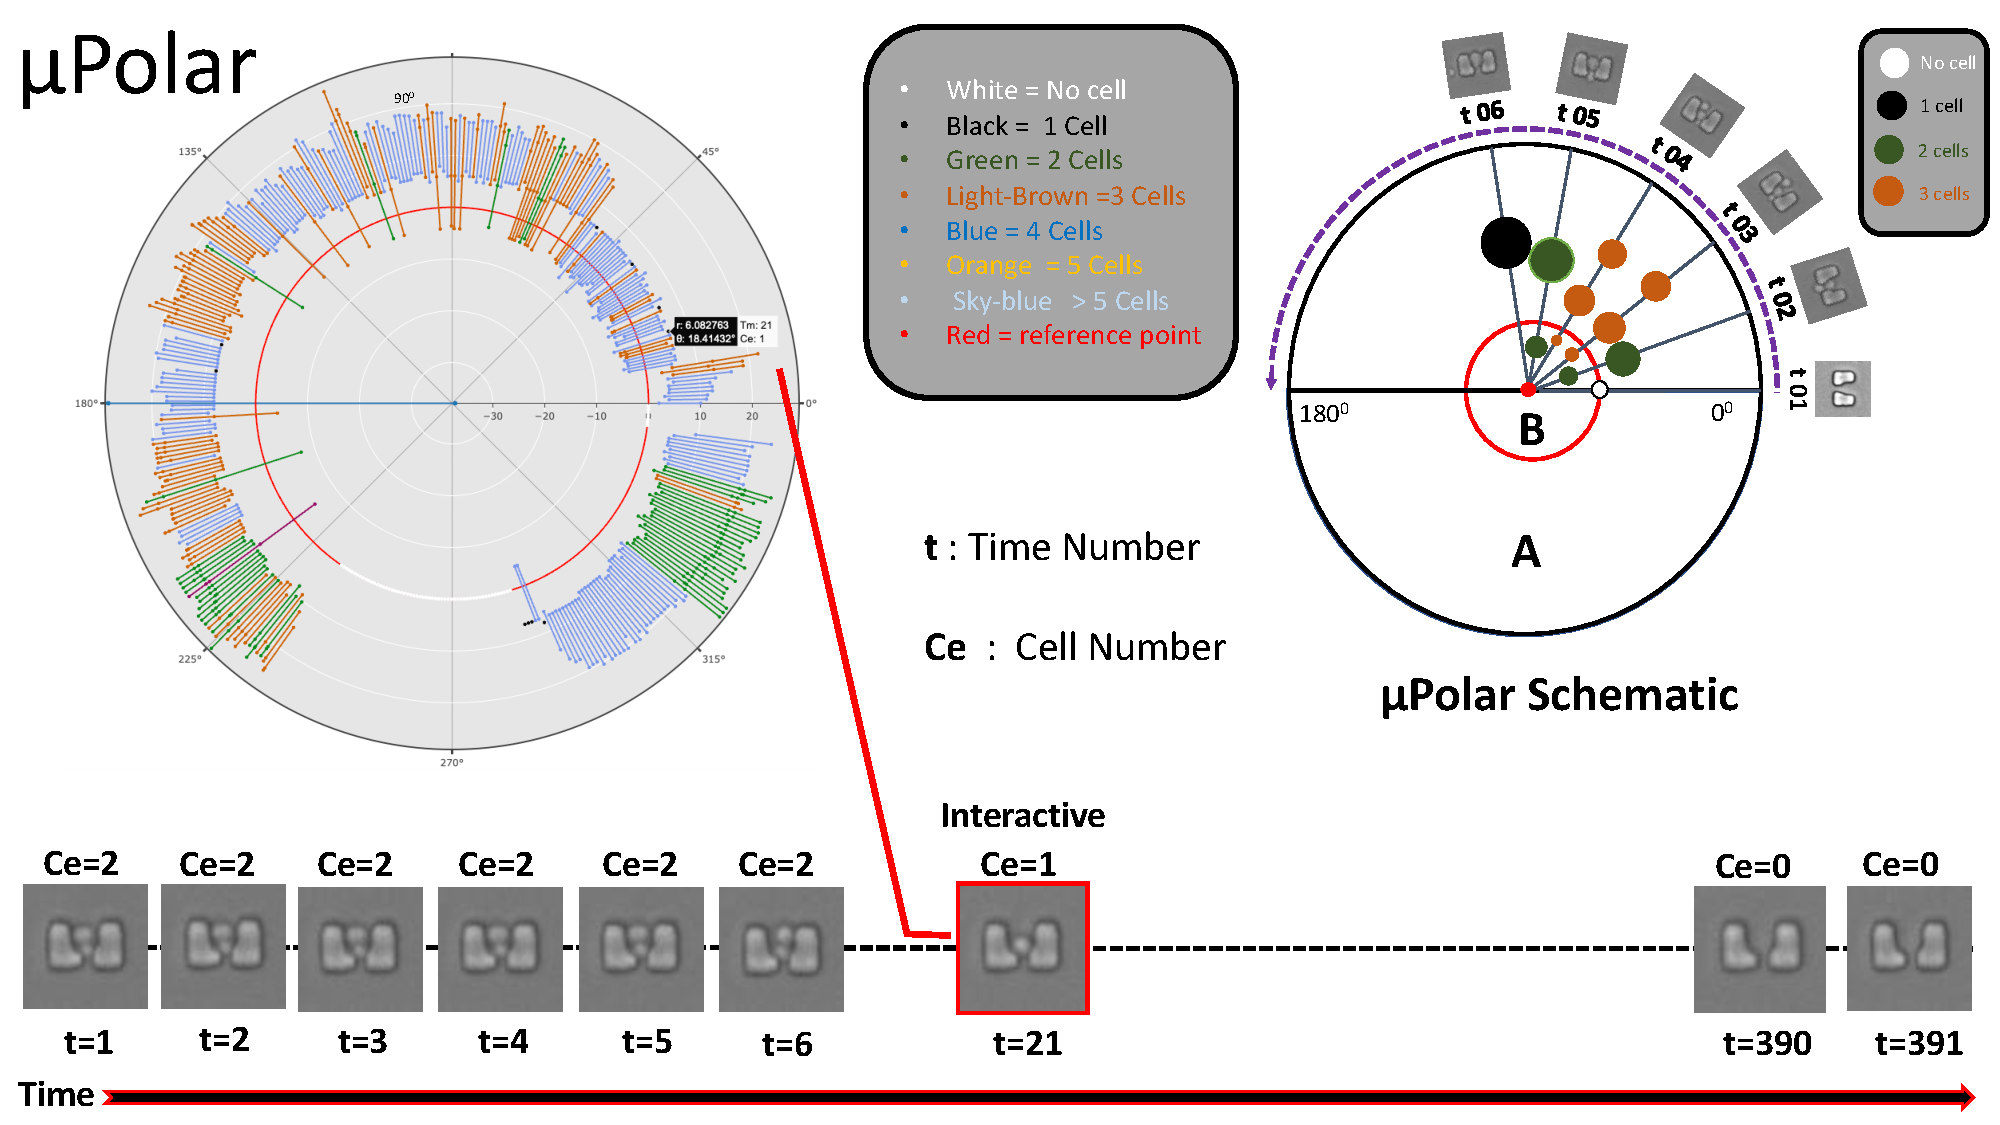
\includegraphics[width=\textwidth,height=10 cm]{Patterns/polar.pdf}
\caption{ \textbf{ A sequence of microfluidic images and dataset formation including $\mu$Polar schematic plot}. (a) Microfluidic sub-images (60x60) labeled with cell number, cell boundary area and reference point. (b) A sample of $\mu$Polar dataset format with optional features of area and RLS. From left to right, column one represents image time-point, column two represents cell centroid point (x, y), column three represents individual cell area and column four represents RLS data for any potential division. (c) $\mu$Polar plot with representation of cell location on the plot and cell color tag. }
\label{fig:table}
\end{figure*}
\

\subsubsection{Distance calculation}
Since the cell time-point, coordinate and area (optional) are available from dataset (e.g. Fig.\ref{fig:table}b), the cell distance can be calculated from reference point by using the Euclidean equation:

\begin{equation}
\begin{split}
d_i = \sqrt{(x_i - x_r)^2 + (y_i - y_r)^2}\\
\\
i =  [1,2,3,4,..., m ] \\
\\
\end{split}
\end{equation}

where $ d_i $ is the distance between the centroid point of cell and given reference point as shown in Fig.\ref{fig:table}a (blue lines). $ x_i $ and $ y_i $ are cell coordinate at each image. $ x_r $ and $ y_r $ are given reference point which needs to be specified by user when is running the $\mu$Polar function. $ i $ is the image number corresponding to the time-point and $ m $ is the maximum time-point equivalent to the total number of images. In general, reference point could be chosen at any point of image based on the region of interest. For instance, in Fig.\ref{fig:table}a , the reference point (X\_{ref}, Y\_{ref}) was chosen at $x = 30$ and $y = 1$ . This is based on cell movement and the position of the trap. 
\\

\subsubsection{Time-point conversion}
The next step is to convert time-point (number of image) to degree, suitable for circular plot visualization. The time to degree conversion is  calculated by: 

\begin{equation}
%\begin{split}
%\\
\theta = \frac{D_{max}} {T_{max}}
%\\
%\end{split}
\end{equation}

\begin{equation}
%\begin{split}
%\\
A_{acc} = \sum_{i=1}^{n}{\theta_i}
%\\
%\end{split}
\end{equation}

where $ D_{max} $ is the maximum degree (360 degree) and  $ T_{max} $ is the maximum time-point (e.g. last time-point). The  $ A_{acc} $ is accumulative angles of each radius vector ($\theta$) and $ n $ is equal to maximum degree. All cell distance values at each time-point are mapped on radius of circular plot with corresponding $A_{acc}$ value.
\\
The $\mu$Polar schematic plot is represented in Fig.\ref{fig:table}c. It illustrates microfluidic images at time-point 1 (zero cell), time-point 10 (one cell), time-point 20 (two cells), time-point 30 (three cells) and time-point 40 (two cells). The color tag method represents the number of cell corresponding to the number of cell(s) in the image. This approach is useful to identify the potential mother cell and daughter cell , and track down the cell movement including the division point. 

%cell movement interpretation. 
%%%%%%%%%%%%%%%%  how to pick reference point    $$$$$$$$$$$$$$$$$$
%We decided to choose the reference point based on cell flow direction and potential cell division point.
%Here, $ x_r $ and $ y_r $ are set to be 30 and 34 respectively at trap outlet as shown in $\nameref{S1_Fig}$. 


 %time-lapse microfluidics-based microscopic to a circular plot based on the image time and the cell distance in 2D. 
 
 % this is NOT accurate. uPloar does not detect cell objects from images
 
 % remove quotes, use italics
 
 
%Polar package, written in R language, utilizes three other R libraries, tidyverse, utils and plotly. The input of Polar are cell objects identifications, coordinates, movement measures, and timestamps. The Polar function takes time-lapse ”dataset” which only requires image ”time” and cell ”coordinate”. The dataset should be in comma-separated values (csv) format with at least ”time” and ”coordinate” features. ”Area” and ”RLS” data also could be used as additional features for the Polar visualization. Fig.1a shows a sub-image of microfluidic image (60x60) with four yeast cells inside the trap. Each cell is represented with a number and an area (circled in black). The ”red dot” represents the reference point to calculate Euclidean distance. The reference point can be chosen by the user based on investigation and limited by image dimension. Fig.1b represents the features of the dataset containing image ”time” and cell ”coordinate”. The ”area” and ”RLS ” attributes can be optionally visualized for cell monitoring and RLS analysis. In addition, Polar offers a color-based cell tracking option for cell tracking visualization.
 

%%%%%%%%%%%%%%%%%%%%%%%%%%% available color %%%%%%%%%%%%%%%%%%%
%%The $\mu$Polar" color codes are set up for 12 colors  by default categorizing the number of available cells at each time-point corresponding to cells distance. Any number above 12 would be presented as a random color. The color codes are adjustable and could be varied for different image types.  
 
 
\subsection{$\mu$Polar function}
The $\mu$Polar package, written in R language, utilizes three other R libraries including \textbf{\textit{tidyverse}}, \textbf{\textit{utils}}, \textbf{\textit{plotly}}. The $\mu$Polar function has 11 arguments where the first argument is the input dataset and the remaining arguments are required for visualization adjustment. Table. \ref{table:desc} demonstrates an overview of $\mu$Polar function arguments. (I) argument is the time-lapse dataset and should include \textbf{\textit{time}} and \textbf{\textit{coordinate}} which are required for basic visualization. The \textbf{\textit{Area}} and \textbf{\textit{RLS}} are optional features of the $\mu$Plot function which can be added to visualization results if they are available from dataset. (II) the argument is the reference point (x, y) that can be chosen by the user. The reference point mainly depends on the type of image and the purpose of the investigation (e.g. edge coordinate of image in direction of cells movement). (III) the argument is to select a particular range of time-points for plot visualization. The starting and ending time-points can be given by the user, otherwise, $\mu$Polar visualizes all time-points. This is useful to analyze a specific range of time-points (e.g. overcrowded cells). (IV) the argument displays the plot title, otherwise the default is non-title. (V) the argument is to evenly divide angle line on the plot. This is also useful to analyze a range of time-points when there is an overcrowded region on the plot. (VI) argument is to set the format for each divided angle (e.g. text format), otherwise it would be in degree format. (VII) the argument are numerical values (X\_{ref}, Y\_{ref}) indicating the reference point on the image. which used to calculate the cell distance. (VIII) argument is to activate cell area dataset  when is available. It represents cell with actual size which is useful to visualize cell movement interpretation. (IX) the argument is to adjust cell size when the cell area dataset available which is useful fr cells overcrowded situation. (X) the argument is to activate the color tracking , and the default is set to 12 colors. This is en effective option to visualize cell tracking identification at each time-pints. In addition, it is very beneficial for RLS analysis when the cell development can be visualized based on cell size over the time. (XI) the argument is to adjust the cell distance from the edge of plot when there is an overcrowded situation. 


%\begin{figure*}
%%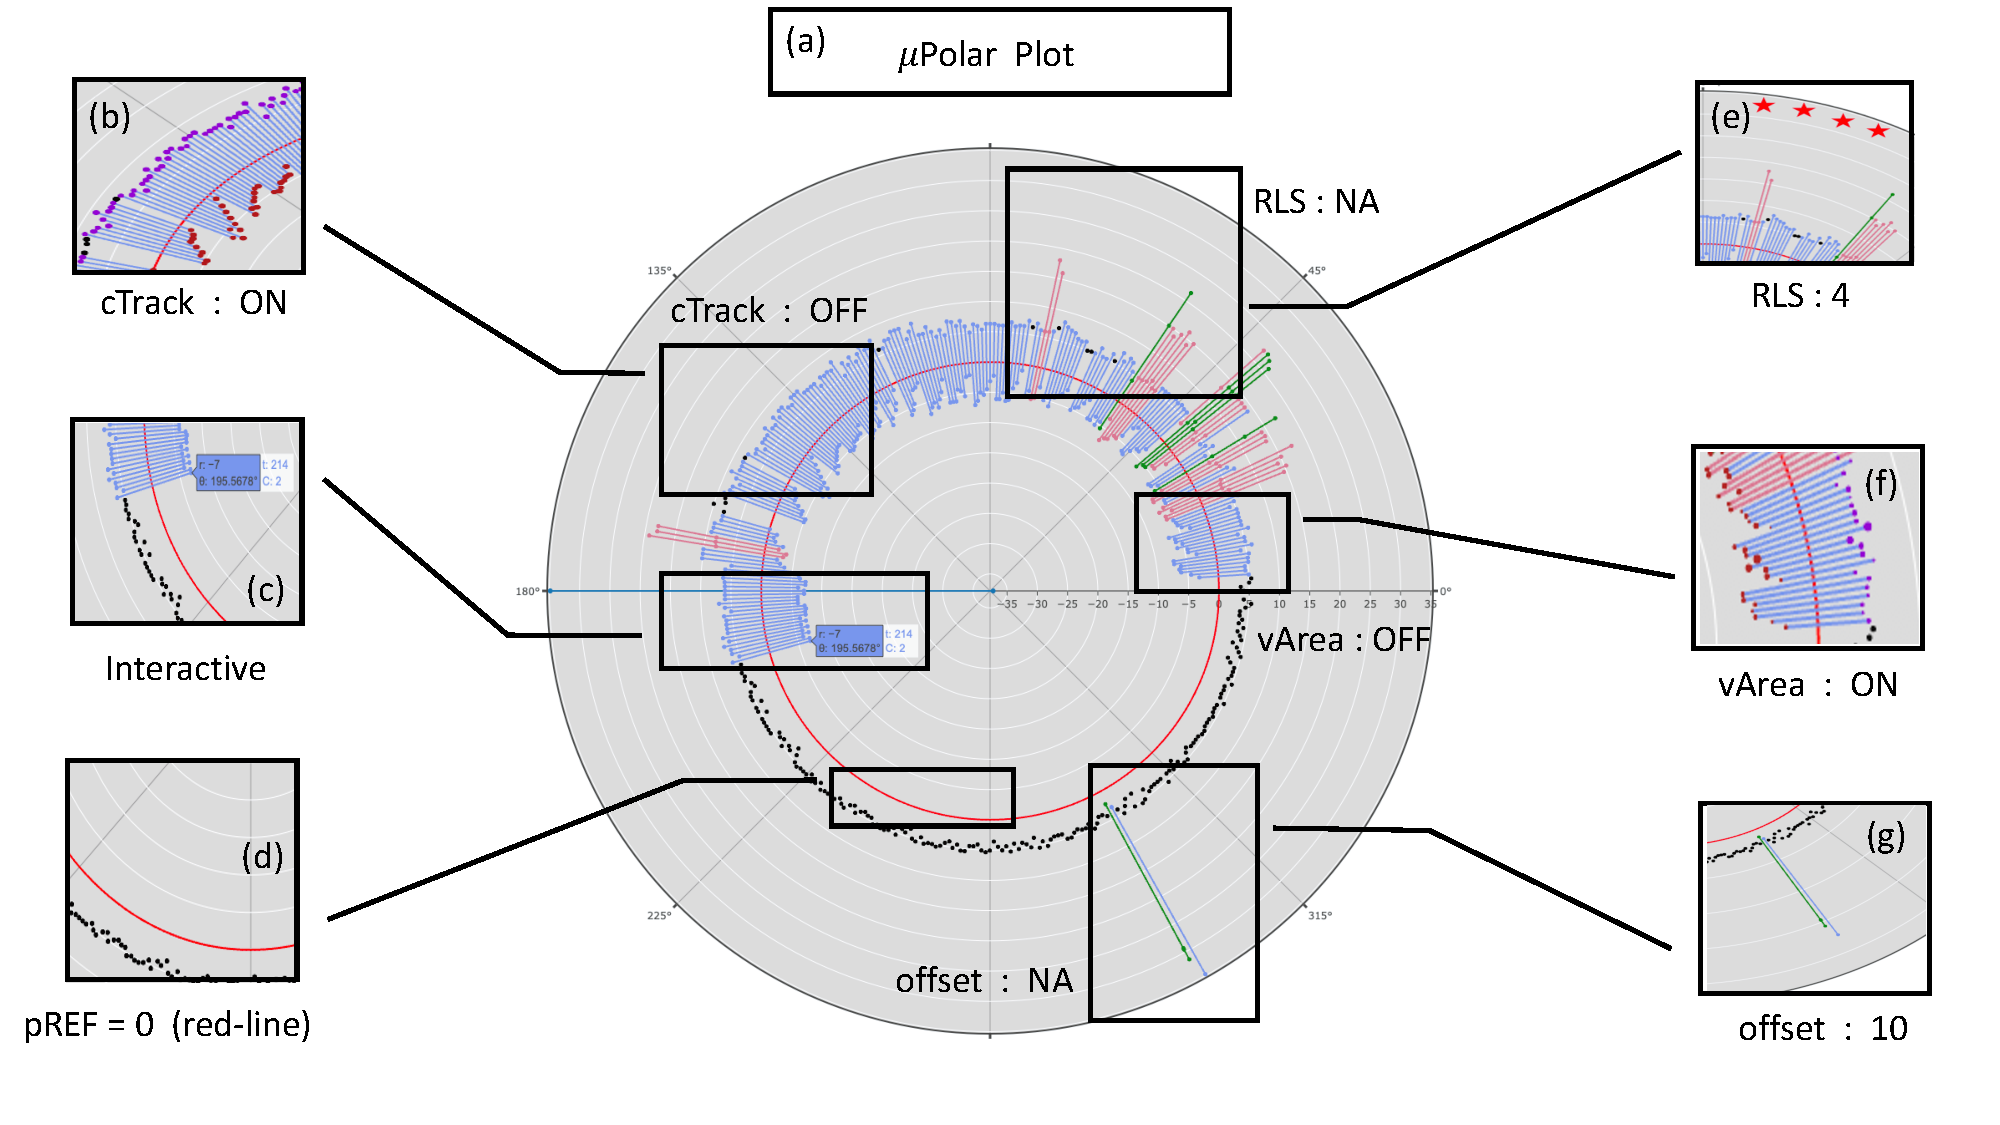
\includegraphics[width=\textwidth,height=10 cm]{Patterns/function_argu.pdf}
%\caption{ \textbf{ $\mu$Polar function inputs, time, distance, area, offset, adjust, track, and RLS}. (a) It is the $\mu$Polar plot title. (b) It shows $\mu$Polar color tracking activation when is OFF or ON. (c) It represents an interactive option in $\mu$Polar plot. (d) It illustrates the given plot reference line on the $\mu$Polar plot. (e) The RLS is available from the dataset and represented by "red star" (RLS = 4). (f) The comparison of vector area of cells when they are available from the dataset. (g) The adjustable option when cell distance is close to the edge of the plot %(offset = 10).}
%\label{fig:label}
%\end{figure*}


\begin{table*}[ht]
\caption{$\mu$Polar function description}
\centering
\begin{tabular}{p{0.3\linewidth}p{0.1\linewidth}p{0.5\linewidth}}
\\ 
\textbf{Function}\\
\\
\hline
\hline
\\
$\mu$Polar(data,dREF,tmPoint,titile,numAtics,AticFmt,pREF,vArea,sAdjust,cTrack,eAdjust)\\
\\
\hline
\hline
\\
\textbf{Number} & \textbf{Argument}  &\textbf{Description}\\
\\
\hline
\hline
\\
(I) & data &       Input dataset containing Time, coordinate, Area (optional) and RLS (optional)\\
\\
(II) & dREF &      Given reference point (X\_{ref}, Y\_{ref}) \\
\\
(III)& tmPoint &   Given starting time-point and ending time-point\\
\\
(IV)& title &      Given title (default = no title)\\
\\
(V)& numAtics &    Number of evenly spaced angle\\
\\
(VI)& AticFmt &    foramt angle to text (e.g. $T= \%2.2f $)\\
\\
(VII)& pREF &      plot reference line \\
\\
(VIII)& vArea &    Vector cell when areais available (Active: ON ) \\
\\
(IX& sAdjust &     Adjust cells size\\
\\
(X)& cTrack &      Color vector for color tag tracking (Active:  ON)\\
\\
(XI)& eAdjust &    adjust plot edge to cell distance\\
\\
\end{tabular}
\label{table:desc}
\end{table*}


\subsection{Understand $\mu$Polar plot}
To have a better understanding of the $\mu$Polar visualization, there are key points that need to be considered for $\mu$Polar plot analyzes. Fig.\ref{fig:read} is an overview of some prevalent events from time-lapse microfluidic images of yeast cells. Each of the sub-figures is a representation of the most common visualization events generated by $\mu$Polar. For example, the black arrow in Fig.\ref{fig:read}a pointing white dot color is representing the time-point without any cell representation at corresponding microfluidic image. It commonly occurs due to shortening the cell life-cycle. The event in Fig.\ref{fig:read}b portends the upcoming division event (pointing black arrows) from potentially mother cell (mC) located inside the trap with a bud at the trap outlet (see the corresponding image). The red line represents the reference point located at the trap outlet, the purple dot represents mC that located inside the trap (see the corresponding image) and the dark-red dot represents the bud (see the corresponding image). This estimation is based on  visualization of two cells (e.g. mc and bud). In the next event (c), the black dots (pointing black arrows) are representing the single-cell separation cycle that occurred after bud increased in size and the single-cell remains inside the trap (see the corresponding image). The event (d) shows overcrowded events when the number of cells in the image reaches five cells (purple color) where each color is representation of a different number of cells. The (e) and (f) events are good visualization examples of cell size development over time which determinate the occurrence of cell division. In the event (e), the arrow in the up region indicates that the single-cell inside the trap (black dot) started division and there is not much cell development. In fact, the cell (block dot) remains in steady position and after the cell division, the same cell represented by the purple dot. However, the two arrows in the down reg ion indicate that there is a daughter cell (dC) that represented by dark-red dot, attached to the mC and gradually growing in size until complete its division cycle. The event (f) illustrates similar development in the opposite cell flow direction (above reference point) when a mC is located inside the trap in a steady position and the cell above it is growing gradually. These two events are very important to distinguish the division points when the is not any representation of a single cell for counting RLS. The event (g) demonstrates an event that two cells that have been close to each other for some time without much cell size development. These events are considered as senescence time-points of cells. The event (h) shows a single cell inside the trap has been in a steady position for some time. This most commonly happened at the end of the cell life cycle and is considered as a dead cell.


\begin{figure*}
\centering
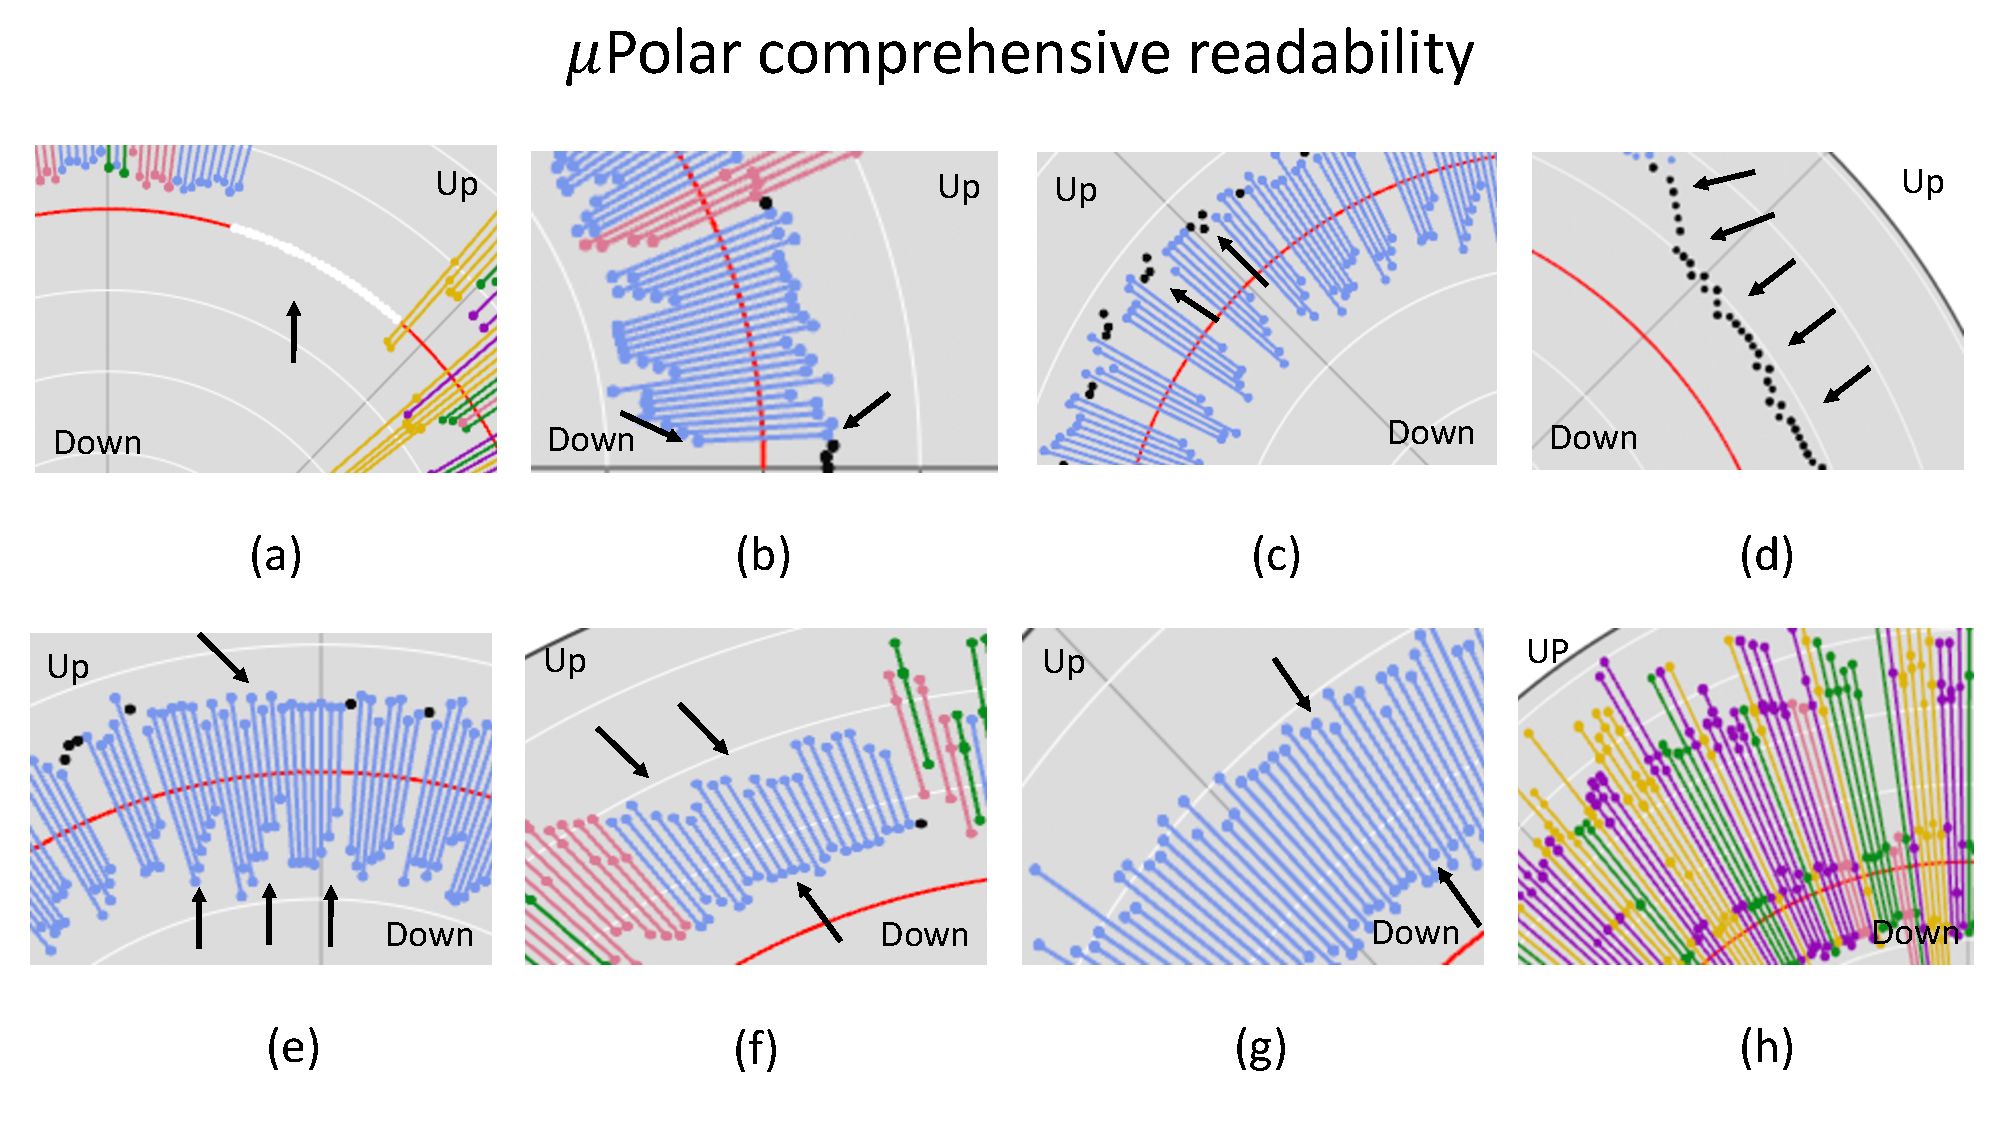
\includegraphics[width=\textwidth,height=10 cm]{Patterns/read.pdf}
\caption{\textbf{ $\mu$Polar plot for some comment visualization events}. Any events occurred below the reference line (red) denoted as "down" and any events occurred above the reference line (red) denoted as "up". (a) There is no cell at the presented time(white dots). (b) The two cells presented by  drak-red dot and purple dot are close to each other and division already happened. (c) The black dots are representing a division after two cells completed the separation cycle. (d) Indication of overcrowded cells events. (e) Representation of steady cell in the up region (purple color) and cell development in the down region (dark-red color). (f)  Representation of steady cell in the up region (dark-red color) and cell development the up region (purple color). (g) All cells are in a steady situation for some time, indication of senescence cells. (h) The representation of a single dead for some time.}
\label{fig:read}
\end{figure*}


\section{Package availability}
The package $\mu$Polar is an open source package that is freely available on Github at $<$ https://github.com/merang/uPolar $>$. The package installation can be done in R either using the install\_github function in the ‘devtools’ or using the githubinstall function in the ‘githubinstall’ package. 

%The R code for installation of $\mu$Polar package using the ‘devtools’ package is as follows: \\
%\\
%install.package("tidyvers")\\
%\\
%install.package("R.utils")\\
%\\
%install.package("plotly")\\
%\\
%libarary(devtools) \\
%\\
%install\_github$("https://github.com/merang/uPolar")$\\
%\\


\section{Data collection}
 
We have applied the $\mu$Polar visualization package to two sets of images; time-lapse microfluidic images of yeast cells and time-lapse microscopic images of mouse fibroblasts. The microfluidics sequence images are procured from \cite{ref13} recent experimental work. Since microfluidic images had low resolution (1280x960), we partitioned 391 images to 391 sub-images in 60x60 dimension. For the other dataset, we collected 37 time-lapse microscopic images from \cite{ref05} as a different type of dataset to test on. Since the number of cells in each image (307x306) was more than 50 cells, we cropped a section of time-lapse images in 121x121 dimensions. Base on image size and resolution, $\mu$Polar function can be applied to any time-lapse cellular microscopic images by cropping the region of interest.
\\

Many methods and applications are available to collect cell coordinate and area from selected microscopic images. We used "Fiji - ImageJ" tools to collect cell coordinates and cell area. This process is mainly automatic, however, it may need manual checking for some images with low resolution. Once this process is done, the collected data can be exported as CSV format which is suitable for $\mu$Polar input dataset.  
\\



%%%%%%%%%%%%%%%%%%%%%%%%%%%%%%%%%%%%%
%       add video link for user  
%%%%%%%%%%%%%%%%%%%%%%%%%%%%%%%%%%%%

\section{Results}
%We have applied the $\mu$Polar visualization package to two sets of images; time-lapse microfluidic images of yeast cells and time-lapse microscopic images of mouse fibroblasts. The microfluidics sequence images are procured from \cite{ref13} recent experimental work. Since microfluidic images had low resolution (1280x960), we partitioned the image to time-lapse (1-391) sub-image of 60x60 dimension. Furthermore, we collected 37 time-lapse microscopic images from \cite{ref05} as a different type of dataset to test on. For visualizing the microscopic images, we cropped a section of time-lapse images from 307x306 to 121x121 dimensions. Base on image size and resolution, $\mu$Polar function can be applied to any time-lapse cellular microscopic images by cropping the region of interest.    

% add video link for data collection  %%%%%%%%%%%%%%%%%

\subsection{$\mu$Polar plot for microfluidic images}
Several microfluidic image traps are shown in \nameref{S1_Fig} that included Trap2, Trap12, Trap22, Trap41, Trap50, Trap59, Trap73, Trap82, Trap98 and Trap100. We chose these traps based on the investigation of cell development at the beginning, middle, and end of the microfluidics device. Each color represents several cells in a range of 1 to 6 in individual image. The white, black, light blue, pink, green, purple, orange colors are representing 0 cell, 1 cell, 2 cells, 3 cells, 4 cells, 5 cells, and 6 cells respectively.

we also evaluated some of $\mu$Polar plot from different trap numbers at different time-points with the corresponding image. For instance, \nameref{S2_Fig} shows $\mu$Polar visualization of trap 8 at time-point 109. The plot indicates three cells (pink color) in the image that two cells are above reference point and single-cell is far below the reference point which considered as noise in this image (bottom-right). In another example, the \nameref{S3_Fig} demonstrates trap 33 at time-point 11 when there are two cells available in the image. This is an early stage of cell division when two cells (connected sky blue) are very close to each other.  The \nameref{S4_Fig} illustrates a very interesting $\mu$Polar plot of trap 63 at time-point 340. The image shows that the cell is an early development stage, however, the $\mu$Polar plot indicates that the cell has been at this level for long time and considered as a senescence cell. 


\subsection{$\mu$Polar plot for microscopic images}
 The migrating mouse fibroblasts from microscopic images are  shown in Fig.\ref{fig:scopic}a. The number of available cells in each image is in a range of 50 - 70 depending on the image time-point and the average cell size is bigger then average yeast cell size. For simplicity of the plotting, we worked on a section of these images as illustrated in (Fig.\ref{fig:scopic}b). Correspondingly, feature extraction is applied to these images, collecting cells coordinate of each image in order of time. According to the observation, the cells are gradually migrating from the right side to the left direction of the image over time. Thus, the reference point was chosen at the left-side of the image edge (x = 2, y = 60) for distance calculation. Fig.\ref{fig:scopic}c illustrates the $\mu$Polar plot where the cells number are in a range of 6 - 10 in each time-point and indicated by different color codes. Each color code is representing cell tag with numbers 1 to 10.  


\begin{figure*}
\centering
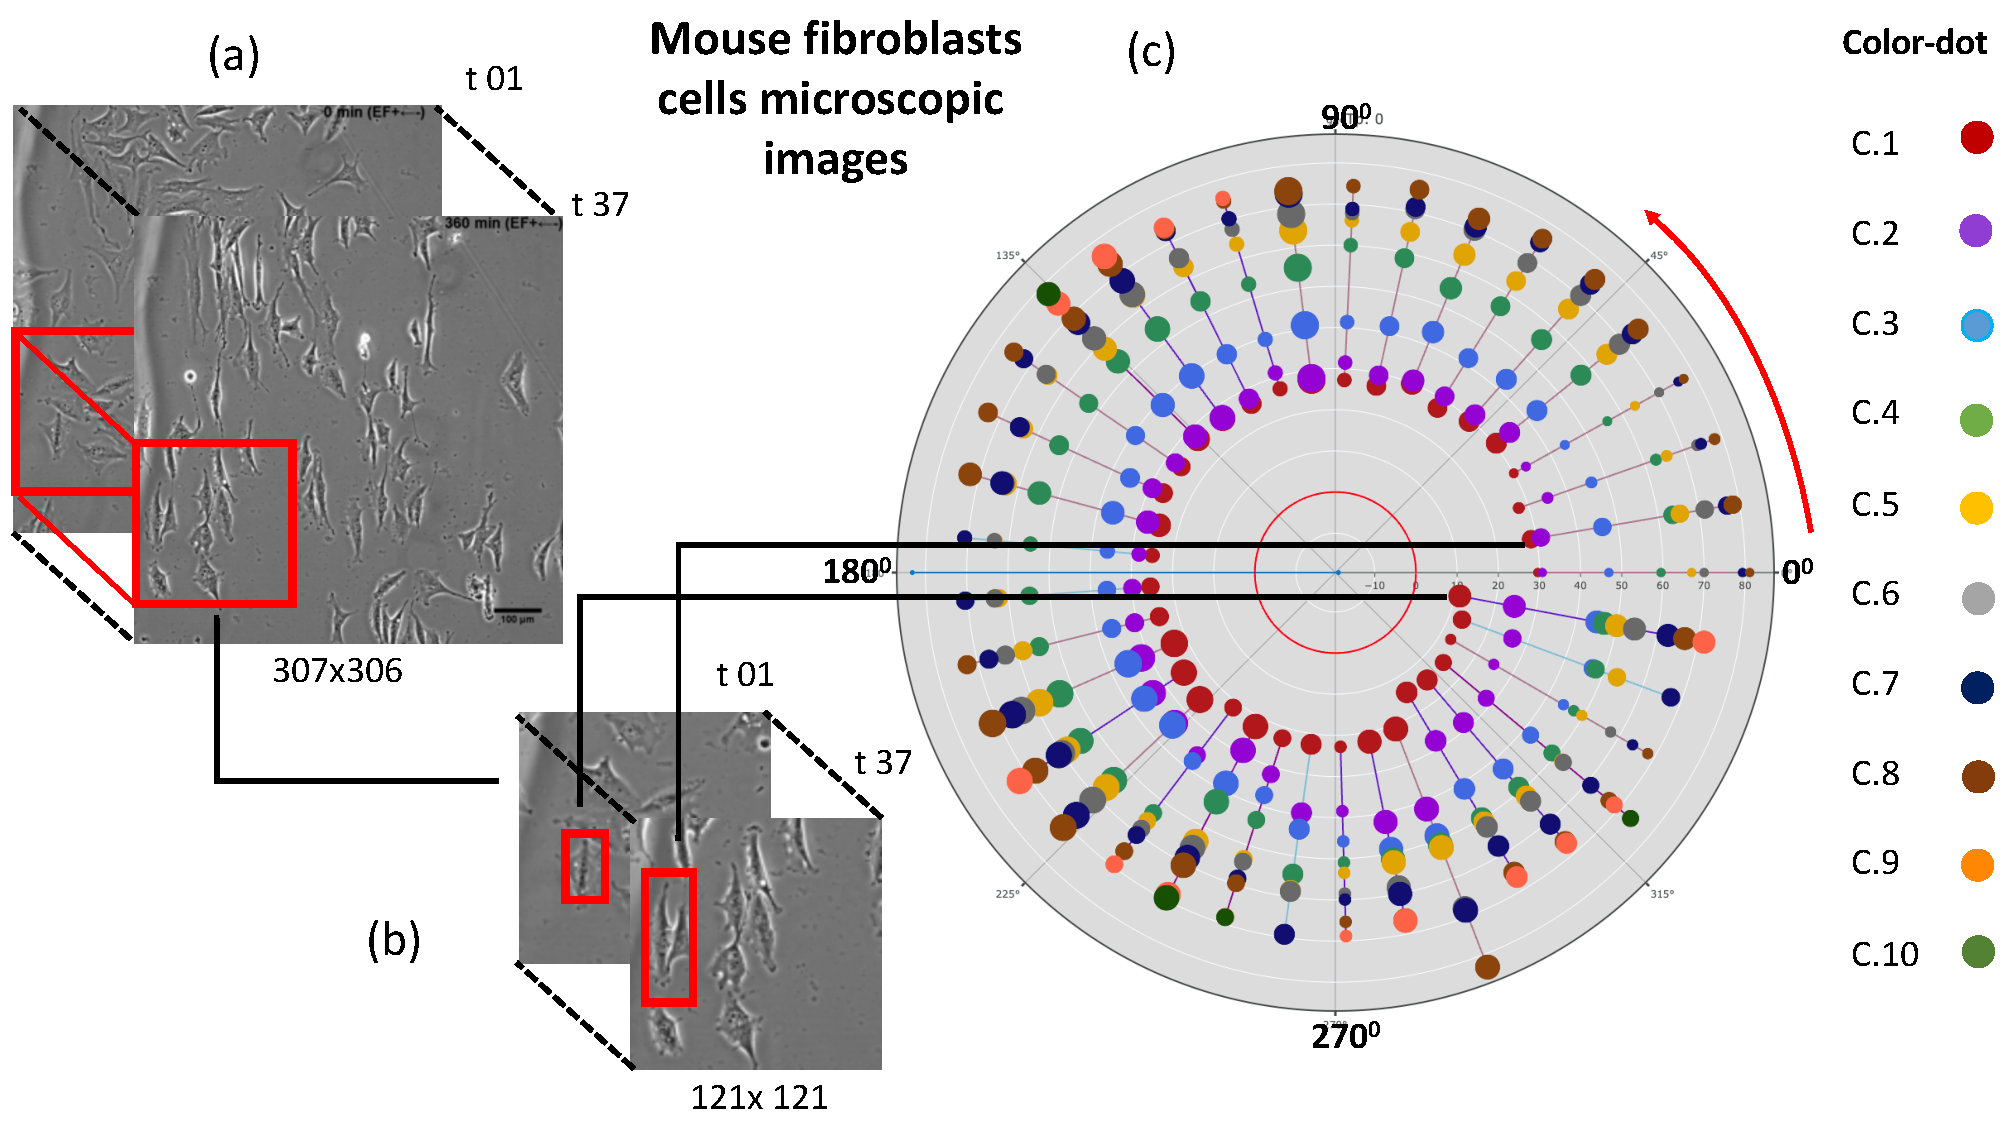
\includegraphics[width=\textwidth,height=10 cm]{Patterns/microscopic.pdf}
\caption{ \textbf{Migration of mouse fibroblasts cells from time-lapse microscopic images applying $\mu$Polar}.}
\label{fig:scopic}
\end{figure*}



\subsection{$\mu$Polar area variation and color tracking }
The cell size variation and movement are important information to understand cell behavior in the aging process. $\mu$Polar function has an option to import cell size information (area) for plot visualization, otherwise, all the cells are represented by default size (5 pixels). The representation of cell variation is very critical to identify the cell division time-points which is very useful for counting RLS.The cell size variation and cell tracking are based on the color tag method in $mu$Polar plot. In general, there are two sets of color representation in $\mu$Polar plot, color-line and color-dot. The color-line is representing the number of cell at each time-point corresponding the number of cell in the image and normally displayed with lighter color. The color-dot is representing cell each time-point corresponding the cell in the image and normally displayed with darker color.

Fig.\ref{fig:scopic}c is a good example of cell size variation. The cell movement and development can be determined by following a cell with same color at each time-points. For instance, the comparison between the closest cell to the center-point at time-point 1 (red) and the closest cell to the plot center-point at time-point 37 (dark-red) shows that the cell migration from time-point 1 to time-point 37 is approximately 20 units. Since the total number of images is 37, $\mu$Polar color tag indication shows a great visualization of cells  movement and size variation. 

Fig.\ref{fig:explain} shows a $\mu$Polar plot when cell area data and color tracking applied to time-lapse microfluidic images. In a quick overview from $\mu$Polar plot,  the number of cell at each time-point is in a range of   2-5 cells. Hence, cells can be tracked down based on color-dot similarity and cell size variation determining the potential division points.
 
 
\begin{figure*}
\centering
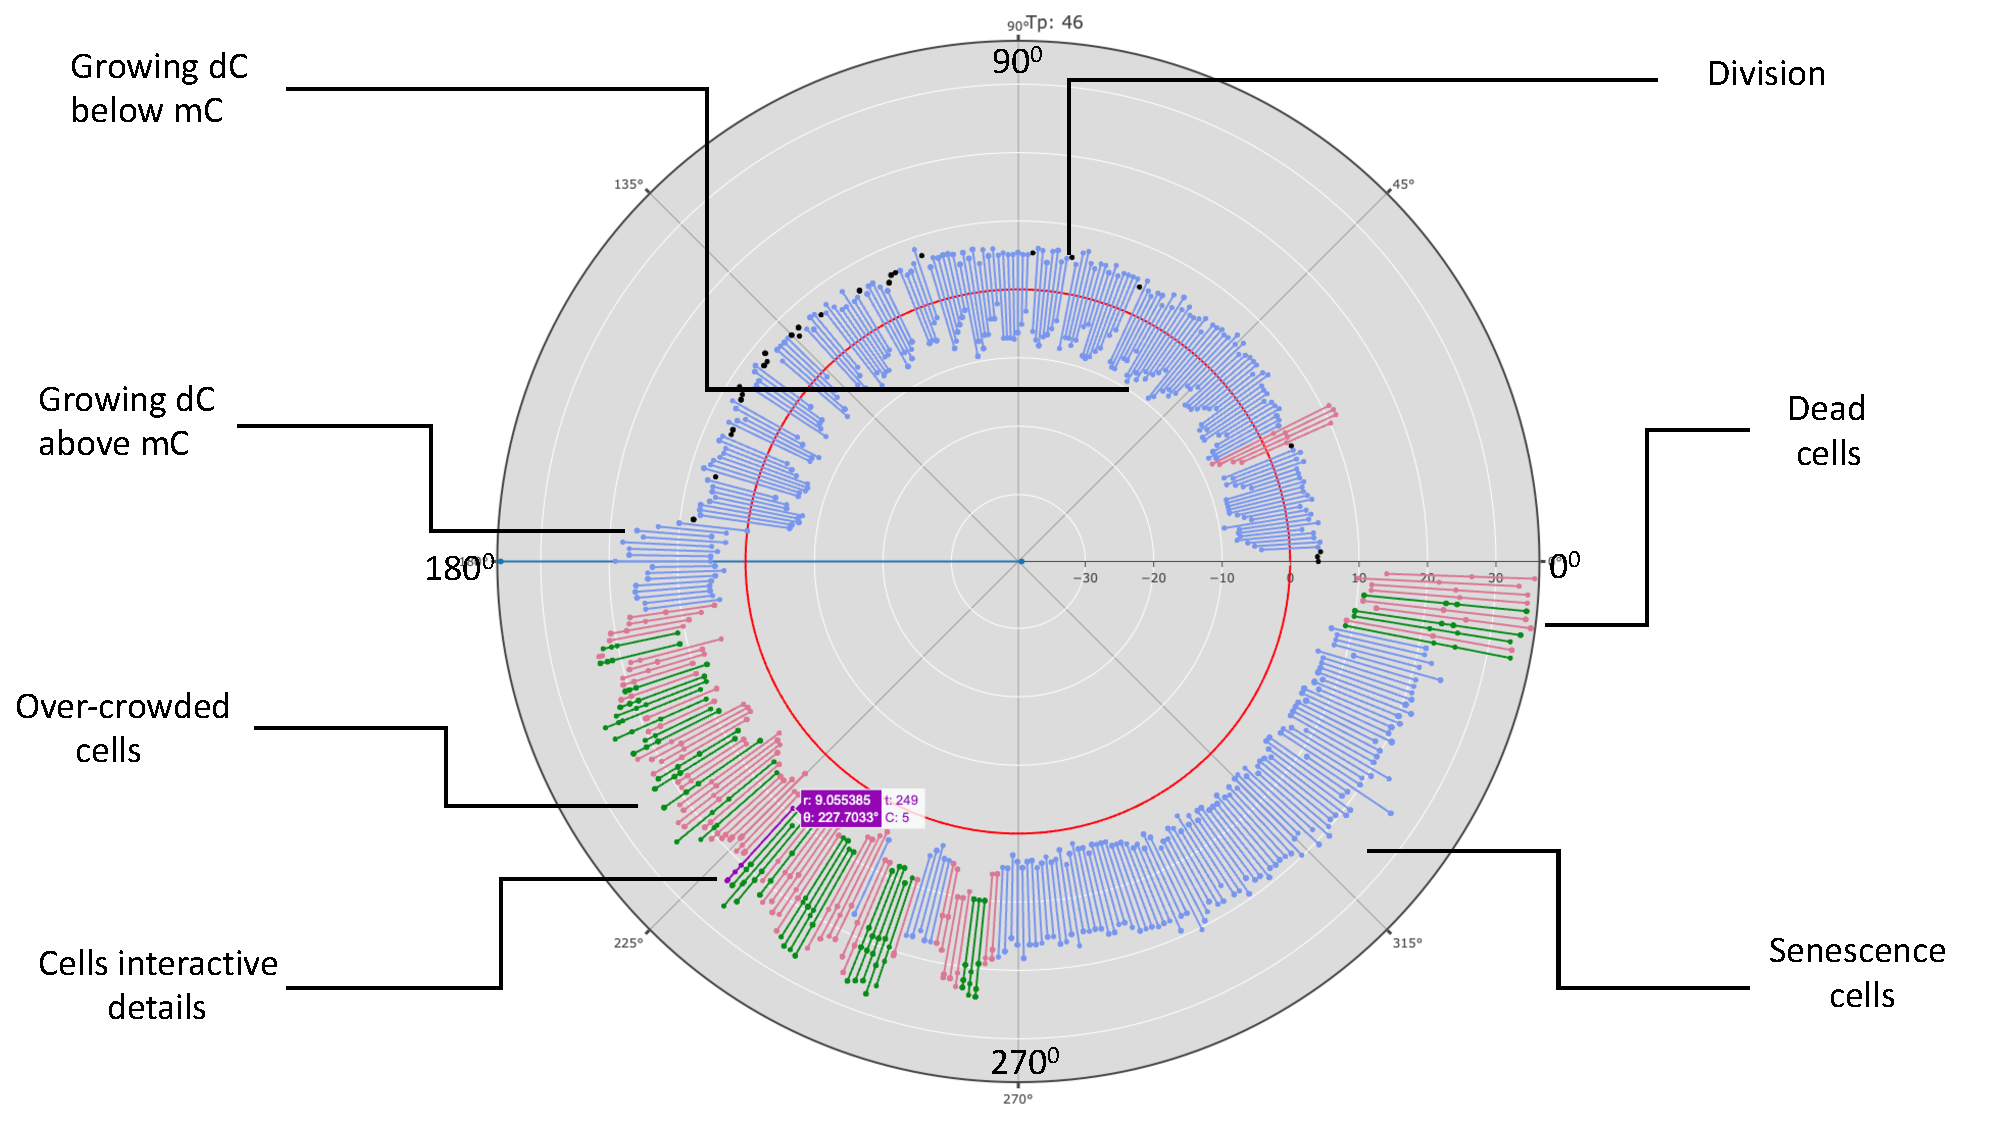
\includegraphics[width=\textwidth,height=10 cm]{Patterns/explain.pdf}
\caption{ \textbf{ $\mu$Polar plot with applied cell area data and color tracking}. The color-lines and color-dots are presenting the number of cells and potential similar color tagged cell at each time-point respectively.}
\label{fig:explain}
\end{figure*}


\subsection{$\mu$Polar RLS counting}
$\mu$Polar has an additional option to visualize the replicative lifespan. This feature could be added to the plot if RLS data is available from the dataset. The RLS division point appears inside the plot out layer with a \textbf{\textit{red star}} color. This feature gives a better understanding of the division point with the corresponding time-points Fig.\ref{fig:rls} demonstrates the RLS comparison between given RLS information and counting RLS from $\mu$Polar plot division points without prior information. We previously collected the experimental RLS data for each trap from \cite{ref02.2} and applied this information to the $\mu$Polar. The $\mu$Polar plot \textbf{\textit{red star}} are representing RLS from experimental results counting 20 division points. The black arrows inside the plot represent the division points from $\mu$Polar plot analysis resulting with counting 21 division points. The estimation is in close range of the  experimental result with an unclear time-point. Although there are some overcrowded time-points and large cells in the second half of the plot, the plot shows the region of interest and range of time-points for counting RLS.       

\begin{figure*}
\centering
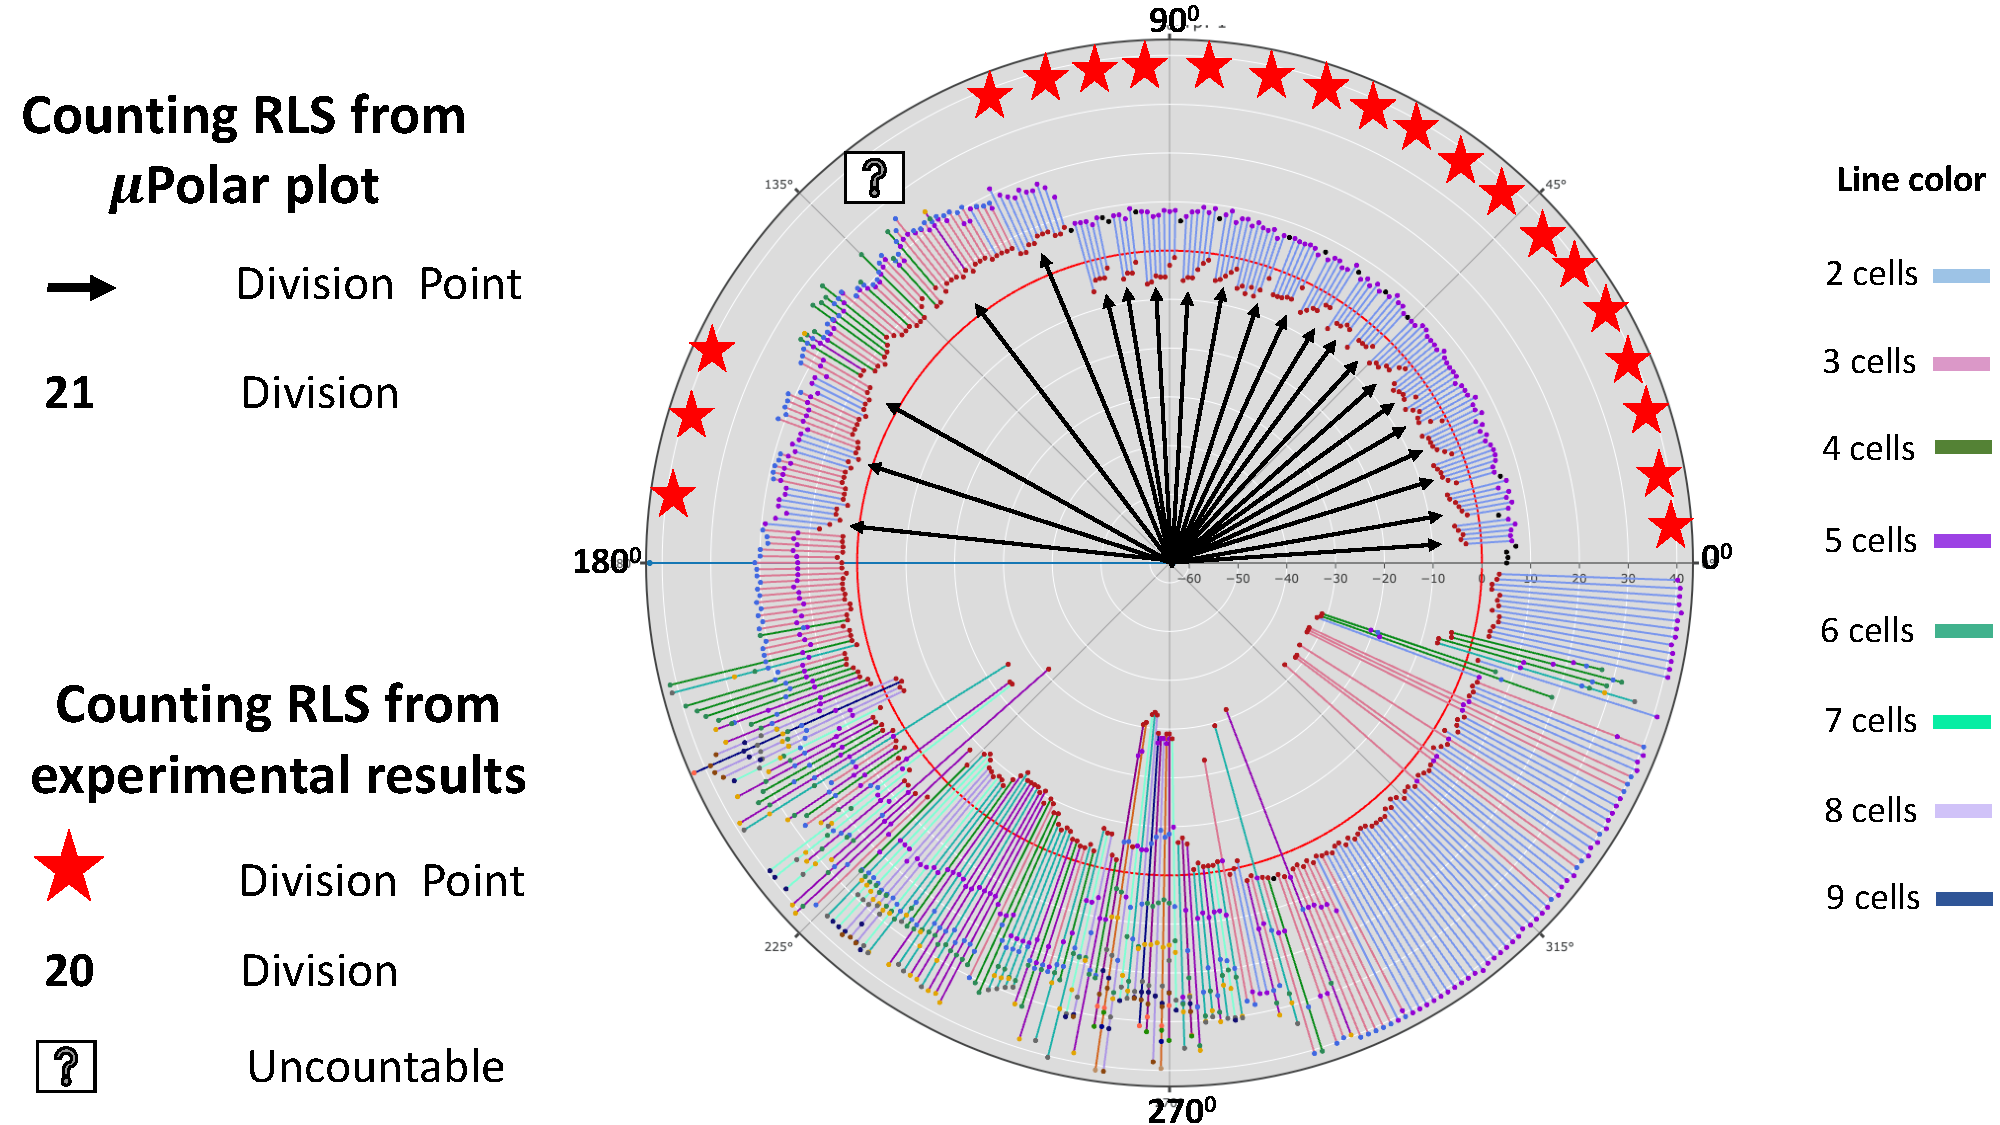
\includegraphics[width=\textwidth,height=10 cm]{Patterns/rlsTp1.pdf}
\caption{ \textbf{Identify the number of RLS from $\mu$Polar}. The "black arrows" are indicating the potential number of yeast cell division time-points from given experimental results (Estimate counting: 21). The "red stars" are indicating the number division time-points that can be identified by $\mu$Polar plot (Estimate counting: 20).}
\label{fig:rls}
\end{figure*}



%In this section, the simplicity and practicality of the $\mu$Polar tool in the contour expansion will be discussed
\section{Discussion}
Fig.\ref{fig:explain} represents Trap98 $\mu$Polar plot from \nameref{S1_Fig}. At first glance, the cell number is in a range of 1-5 cells where black dots represents one cell and color-lines represent two to five cells at each time-point. It appears that the number of cells in the image is two for most of the time-points. The \textbf{\textit{\#1}} event shows that the was a single cell (block dot) in previous time-point and there is a mC (purple dot) with developing bud (dark-red dot) at present time-point, indicating mC at early age. This is \textbf{\textit{dC below mc}} situation, when mC (purple) is inside the trap and dc (dark-red dot) is growing in direction of microfluidic medium flow direction at trap outlet. The \textbf{\textit{\#2}} event illustrates that after some time, there is \textbf{\textit{dC above mc}} situation when single mC(dark-red dot) is inside the trap and dC (purple dot) is developing in opposite direction of microfluidic medium flow direction. The color-dot order is based on closes cell to the plot center point. This can be change from a time-point to time-point, however, similar cells can be identify based on position at theirs time-points. Thus, the purple dot and dark-red dot colors at \textbf{\textit{\#1}} and \textbf{\textit{\#2}} are indicating same mC based on its position on he plot. Between these time-points, there are small variations in the number of cells (color-line) for a short period and followed up by two cells again. This process continued for some time and the number of cells increases (color-line) from two cells to three cells for a longer period until there was not any cell available inside the trap as represented at event \textbf{\textit{\#3}}. After this transition (2 cells to 3 cells), the division started again with \textbf{\textit{dc below mC}} event and continued longer than a similar event at earlier time-points. The \textbf{\textit{\#4}} represents an example of a completed division cycle point from two cells to single cell (black dot). These division cycle points have occurred several times in this example. The division countability  is useful to estimate the number of divisions by visualization. The The \textbf{\textit{\#5}} shows that a dC (dark-red dot) is growing below mC (purple dot). These cells can be tracked down by corresponding color and size variation at each time point.   Cells at overcrowded time-points can also be identified by corresponding color-dots as illustrated in 
The The \textbf{\textit{\#6}}. Senescence time-points at \textbf{\textit{\#7}} are demonstrating that two grown cells (dark-red dot and purple dot) have close to each other for sometimes without noticeable variation in cell size or division point. The The The \textbf{\textit{\#8}} represents a single cell inside the trap close to the end of the experimental work and potentially considered as a dead cell. 

Overall, the $\mu$Polar is a simple and useful tool for visualization of cell migration, cell monitoring, cell development, and cell division estimation from time-lapse microscopic images. The $\mu$Polar interpretation of cell development and comparability at each time-point can be beneficial for identifying division point by visualization which is useful in aging. The comparison between yeast cells time-lapse microfluidics images and mouse fibroblasts cells time-lapse microscopic images demonstrates that $\mu$Polar can be a great tool for visualization time-lapse images with a single plot that includes comprehensive details. For instance, in the microfluidic images, we realized that when cells becoming older over time, interestingly, the cell separation cycle becoming longer and there is a relationship between cell size and separation cycle time.. Similarly, visualizing and tracking mouse fibroblasts cells show that  how cells development over time  and the relationship between cell migration and cell size variation. Potentially, $\mu$Polar could be a great visualization tool to compare a cell separation cycle time at its early lifespan and cell separation cycle time at its late lifespan. Moreover, $\mu$Polar can be useful tool for microfluidic device design and quality evaluation in terms of  trap location and shape. 


\section{Conclusion}
Microfluidics-based microscopy is becoming an increasingly popular research tool to monitor cellular events in biomedical research. One such application is the high-throughput analysis of dividing yeast cells. It is challenging to visualize and interpret the data gathered through microfluidics-based microscopy. Here, we developed a circular plotting method, $\mu$Polar, to visualize cell movements and cellular division events at hundreds of time points. Our method is interactive and easy to use. We demonstrated the utility of our method to describe the events of dividing yeast cells and fibroblasts cells. Our method could be potentially applied to other types of microfluidic devices. This software is implemented in an R package $\mu$Polar available through GitHub from https://github.com/merang/uPolar.

\section{Supplemental Information}

\paragraph*{S1 Fig.}
\label{S1_Fig}
{\bf  Microfluidics traps image visualization using $\mu$Polar R package}. 


\paragraph*{S2 Fig.}
\label{S2_Fig}
{\bf  $\mu$Polar visualization of trap8 with corresponding microfluidics image}. 

% \begin{figure*}
% \centering
% 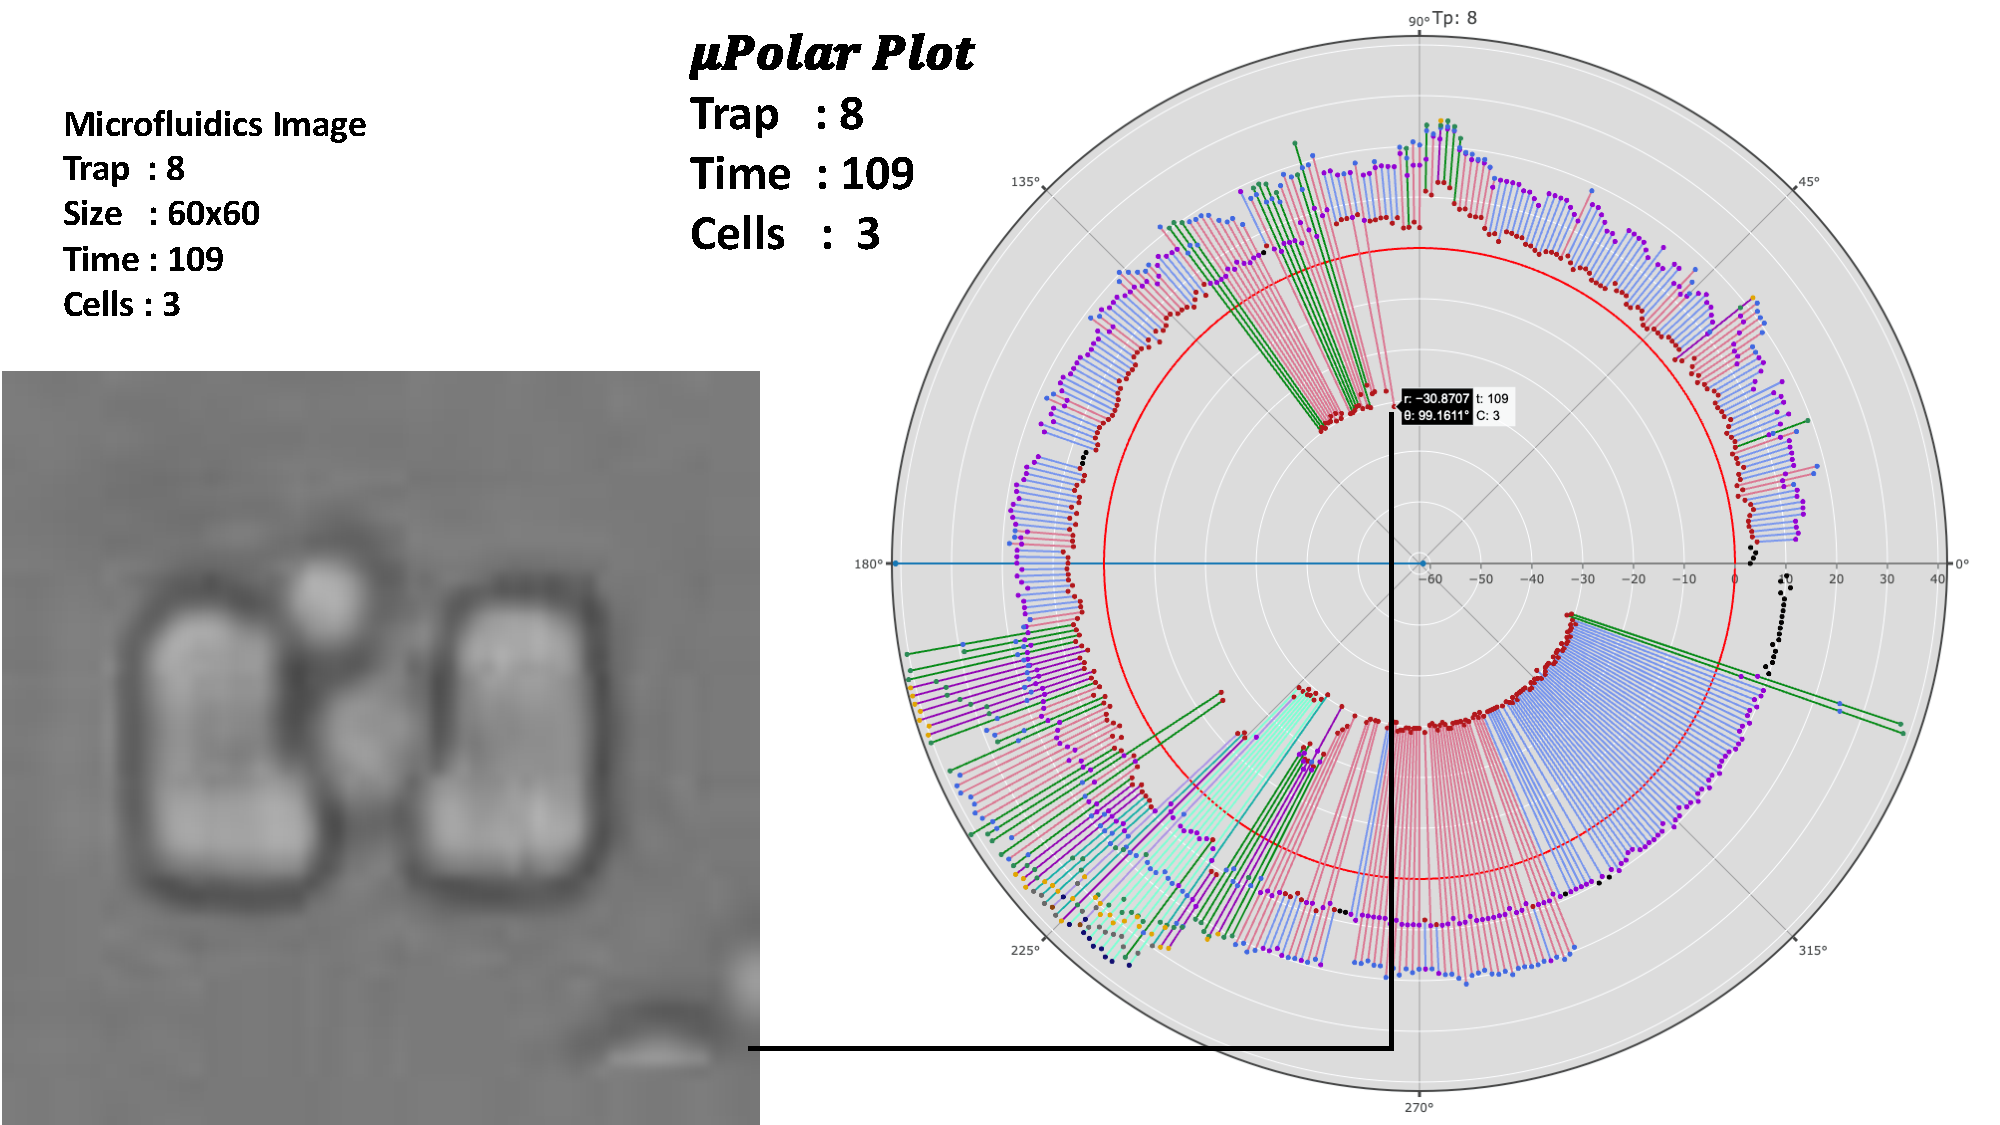
\includegraphics[width=\textwidth,height=10 cm]{Patterns/bc8tp8.pdf}
% \caption{ \textbf{$\mu$Polar visualization for Trap08 microfluidics images}.}
% \label{S1_Fig}
% \end{figure*}

\paragraph*{S3 Fig.}
\label{S3_Fig}
{\bf  visualization of trap33 with corresponding microfluidics image}. 

% \begin{figure*}
% \centering
% 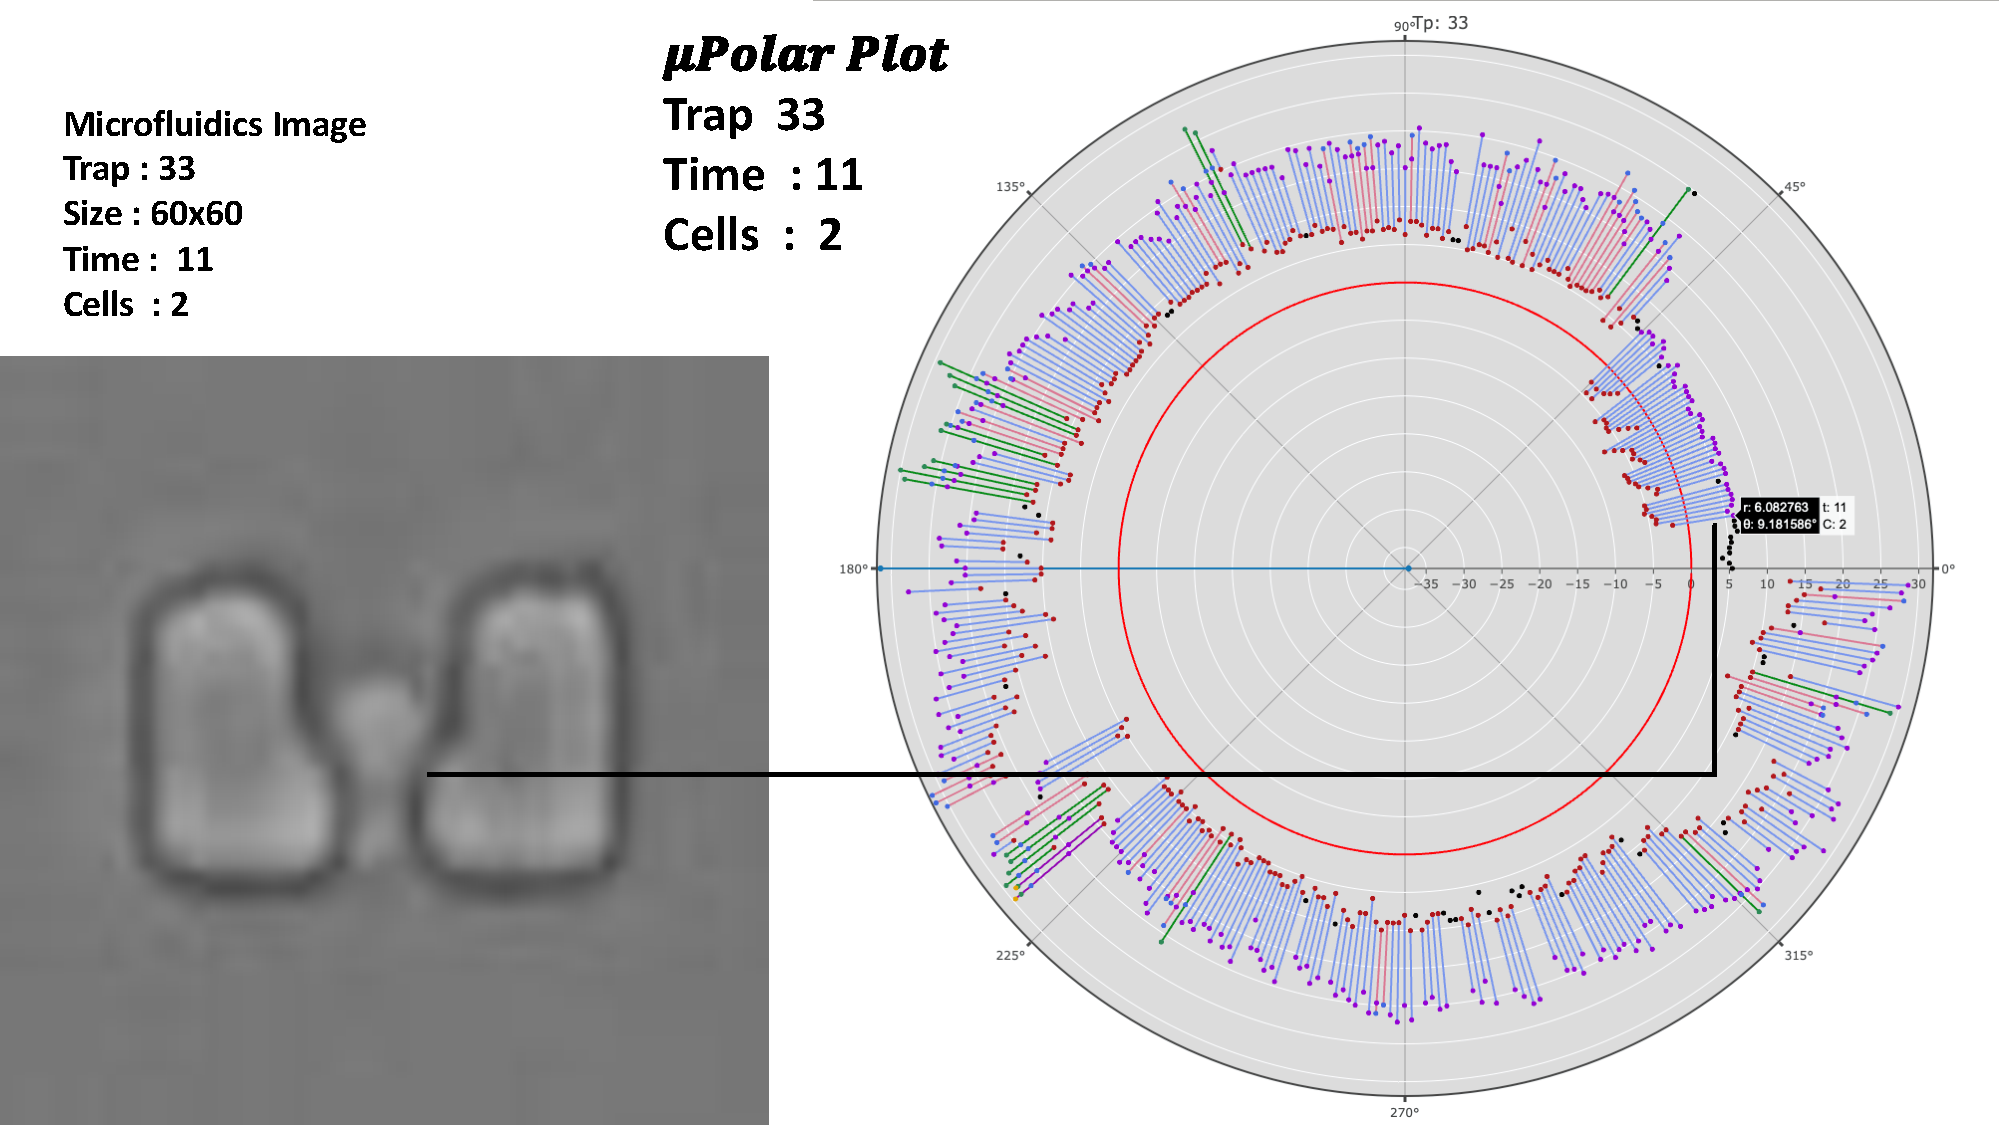
\includegraphics[width=\textwidth,height=10 cm]{Patterns/bc8tp33.pdf}
% \caption{  \textbf{$\mu$Polar visualization for Trap33 microfluidics images}.}
% \label{S2_Fig}
% \end{figure*}


\paragraph*{S4 Fig.}
\label{S4_Fig}
{\bf visualization of trap63 with corresponding microfluidics image}. 

% \begin{figure*}
% \centering
% 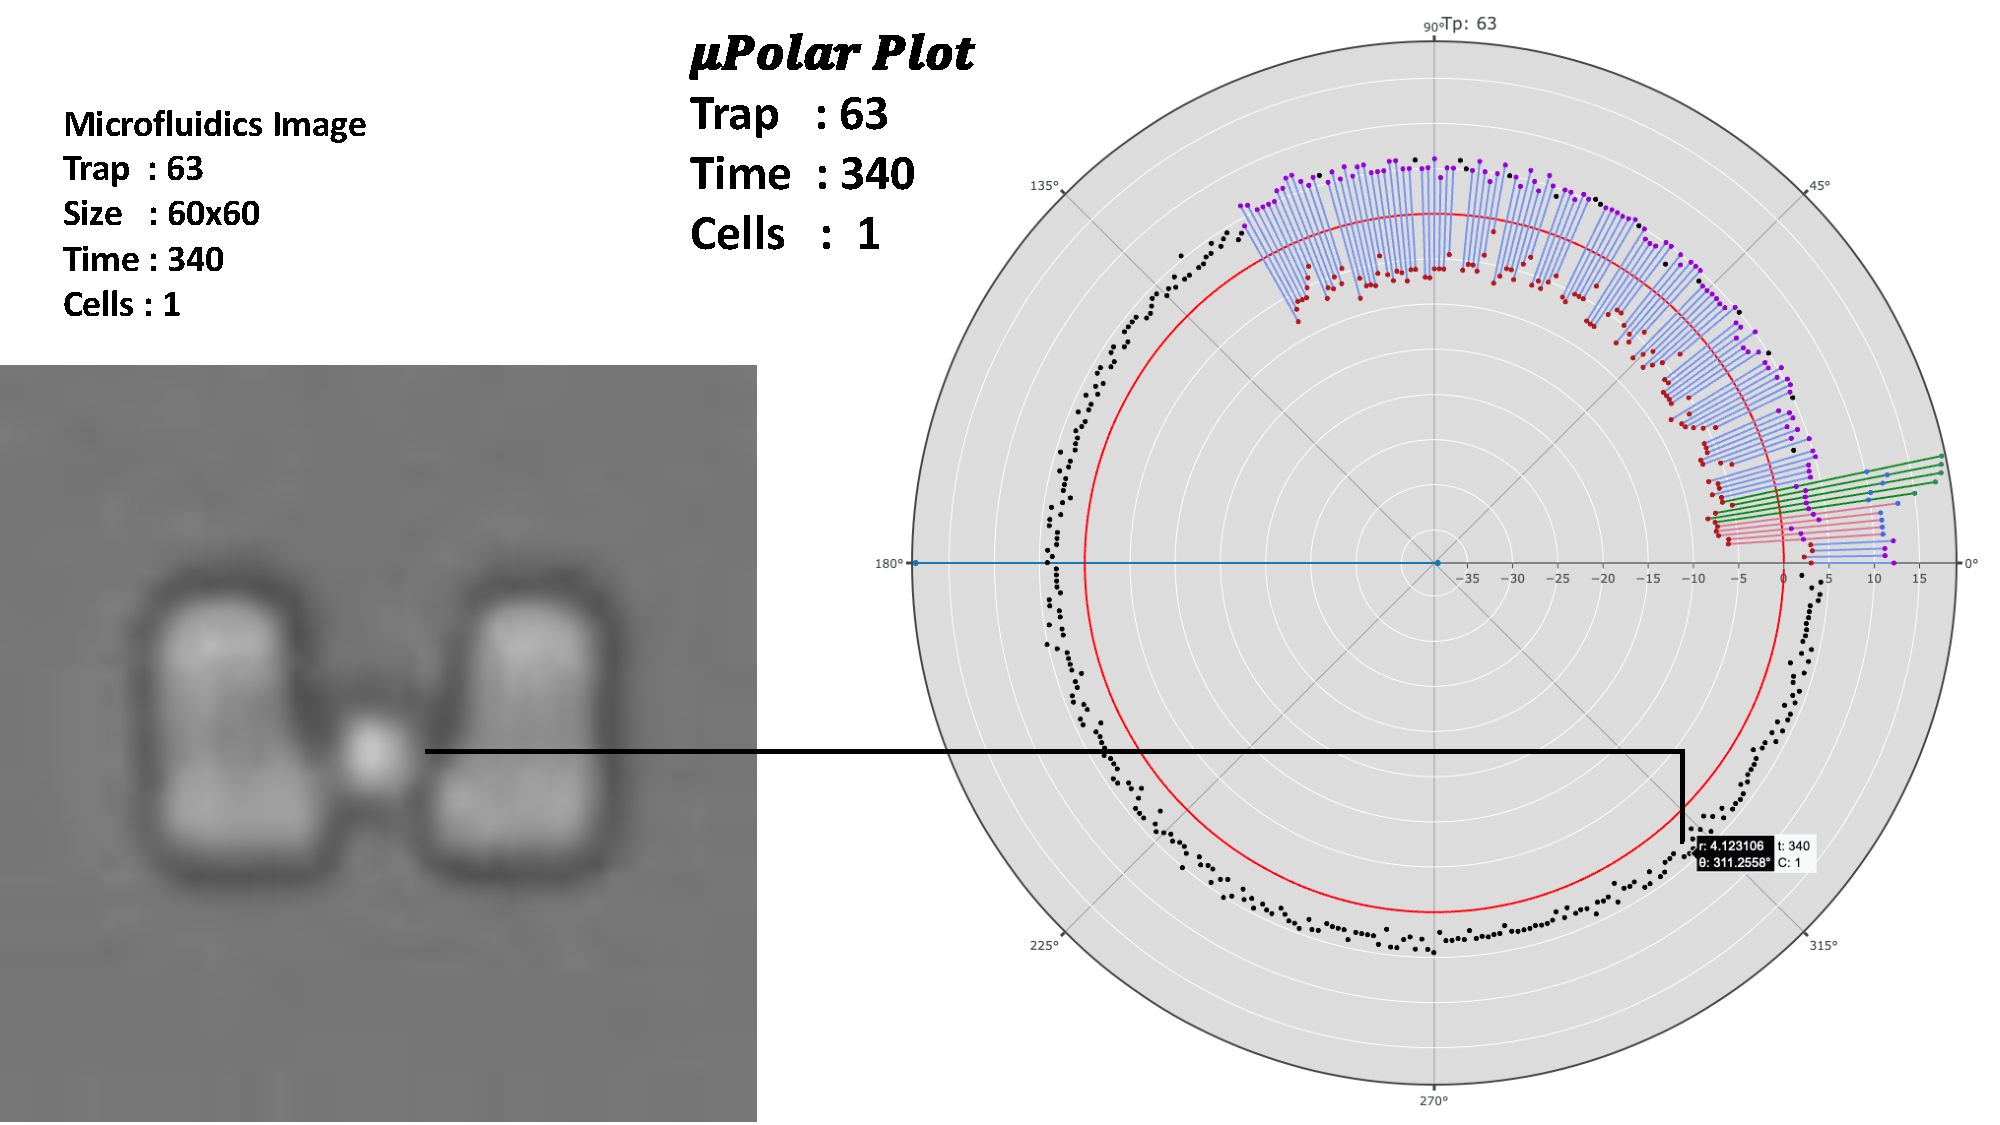
\includegraphics[width=\textwidth,height=10 cm]{Patterns/bc8tp63.pdf}
% \caption{ \textbf{$\mu$Polar visualization for Trap63 microfluidics images}.}
% \label{S4_Fig}
% \end{figure*}



% \begin{figure*}
% \centering
% \includegraphics[width=\textwidth,height=10 cm]{Patterns/fluidics.pdf}
% \caption{ \textbf{HYAA microfluidics chips}. (a) Four modules (16 channels) microfluidic device. (b) A time-point sample of microfludics image shown with guidelines 10 - 70. (c) An example of time-lapse ( t1-t391) images for guidelines 10 - 20. (d) A sample of time-lapse (t1 - t391) partitioned images (60x60).}
% \label{fig:micro}
% \end{figure*}

% \paragraph*{S1 Table.}

% \label{S1_Table}
% {\bf ............} 

\subsection*{Acknowledgment}

The work is partially supported by the NSF CAREER award \#1453078 (transferred to \#1720215), NSF award \#1761839, a  start-up fund, internal CEACSE awards from the University of Tennessee at Chattanooga, and the computing facility of the SimCenter at the University of Tennessee at Chattanooga. We also acknowledge the support of NIH grants \#R01AG052507 and \#R42AG058368.


\subsection*{Author contributions}



\subsection*{Declaration on interests}

The authors declare no competing interests.  

\begin{thebibliography}{00}

\bibitem{r1}

CARPENTERA. E.: Image-based chemical screening.NatureChemical Biology 3, 8 (2007), 461–465


\bibitem{r2}
WOLLMANR., STUURMANN.: High throughput microscopy:From raw images to discoveries.Journal of Cell Science 120,21(2007), 3715–3722

\bibitem{r2.6}
Oates, A. C., Gorfinkiel, N., Gonzalez-Gaitan, M. & Heisenberg, C.-P. Quantitative approaches in developmental biology. Nat. Rev. Genet. 10, 517–530 (2009).


\bibitem{r2.7}
Amat, F. et al. Fast, accurate reconstruction of cell lineages from large-scale fluorescence microscopy data. Nat. Methods 11, 951–958 (2014).

\bibitem{r2.8}
Mavrakis, M., Rikhy, R., Lilly, M. & Lippincott-Schwartz, J. Fluorescence imaging techniques for studying Drosophila embryo development. Curr. Protoc. Cell Biol. 39, 4.18.1–4.18.43 (2008).

\bibitem{r2.9}
Buckingham, M. E. & Meilhac, S. M. Tracing cells for tracking cell lineage and clonal behavior. Dev. Cell 21, 394–409 (2011).

\bibitem{r2.10}
Olivier, N. et al. Cell lineage reconstruction of early zebrafish embryos using label-free nonlinear microscopy. Science 329, 967–971 (2010).


\bibitem{r2.2}
Farokhi H, Ghayesh MH (2018) Nonlinear mechanics of electrically actuated microplates. International Journal of Engineering Science 123: 197-213.

\bibitem{r2.1}
Ghayesh MH (2018) Mechanics of tapered AFG shear-deformable microbeams. Microsystem Technologies 24(4): 1743-1754.


\bibitem{r2.3}
Şimşek M (2016) Nonlinear free vibration of a functionally graded nanobeam using nonlocal strain gradient theory and a novel Hamiltonian approach. International Journal of Engineering Science 105: 12-27.

\bibitem{r2.4}
 Bhagat AAS, Bow H, Hou HW, Tan SJ, Han J, et al. (2010) Microfluidics for cell separation. Med Biol Eng Compu 48: 999-1014.

\bibitem{r2.5}
Shafiee H, Jahangir M, Inci F, Wang S, Willenbrecht RB, et al. (2013) Acute on-chip HIV detection through label-free electrical sensing of viral nano- lysate. Small 9(15): 2553-2563.


\bibitem{r3}
JENSENE. C.: Overview of live-cell imaging: Require-ments and methods used.The Anatomical Record 296, 1 (2013),1–8

\bibitem{ref01}

V. Longo, G. Shadel, M. Kaeberlein and B.  Kennedy, Replicative and Chronological Aging in Saccharomyces cerevisiae, Cell Metabolism, 2002,16(1):18-31.


\bibitem{ref02}
R. Eilsand and C. Athale, Computational imaging in cell biology, Cell Biol.2003, 16: 477-48.

\bibitem{ref02.2}
M. Ghafari,  et al. , Prototyping a family tree algorithm to estimate yeast replicative lifespan from time-lapse microfluidic images, IEEESouthEastConf. 2020, (awaiting for publication)


\bibitem{ref03}
D. Webb and A. Horwitz, New dimensions in cell migration, Cell Biol, 2003,  5: 690-692.

% \bibitem{ref04}
% M. Kaeberlein, K. Kirkland, S. Fields and B. Kennedy, Sir2-Independent Life Span Extension by Calorie Restriction in Yeast, PLoS Biology,,2004, 2(9):e296.

\bibitem{ref4.2}
H. Qin, Estimating network changes from lifespan measurements using a parsimonious gene network model of cellular aging, BMC Bioinformatics 20, 599 ,2019, doi:10.1186/s12859-019-3177-7









\bibitem{ref05}
H. Tsai et .al, Usiigaci: Instance-aware cell tracking in stain-free phase contrast microscopy enabled by machine learnin. 2019, doi.org/10.1016/j.softx.2019.02.007.

\bibi



tem{ref07}

D. Botstein and G. Fink, Yeast: An experimental organism for 21st Century biology. Genetics, 2001, 189(3): 695-704.


\bibitem{ref08}

K. Steffen, B. Kennedy and M Kaeberlein, Measuring replicative life span in the budding yeast, JoVE, 2009,  28: 1-5.

\bibitem{ref09}

M. Kaeberlein and B. Kennedy, Large-scale identification in yeast of conserved ageing genes. Mech Ageing Dev,2005, 126(1):17-21.

\bibitem{ref10}

D. Sinclair, K. Mills, and L. Guarente,  Aging in Saccharomyces cerevisiae, Annu. Rev,  Microbiol, 1998, 52: 533-560.


\bibitem{ref11}

S. Enfors  et al. , Physiological responses to mixing in large scale bioreactors, J Biotechnol,2001, 85: 175-185


\bibitem{ref12}

K. Chen, M. Crane and  M. Kaeberlein, microfluidics Technologies for Yeast Replicative Lifespan Studies. Mechanisms of ageing and development, 2017, 161(Pt B):262-269.


\bibitem{ref13}

 M. Jo, W. Liu, L. Gu, W. Dang and  L. Qin, High-throughput analysis of yeast replicative aging using a microfluidics system, Proc. Nati. Acad. Sci. USA, 2015, 112: 9364-9369.


\bibitem{ref14}

M. McCormick,  J.Delaney, M. Tsuchiya, et alA comprehensive analysis of replicative lifespan in 4,698 single-gene deletion strains uncovers conserved mechanisms of aging, Cell metabolism, 2015, 22(5):895-906.


\bibitem{ref15}
S. Pang,  et al. ,A novel YOLOv3-arch model for identifying cholelithiasis and classifying gallstones on CT images, PLoS ONE, 2019, 14(6): e0217647. https://doi.org/10.1371/journal. pone.021764

\bibitem{ref16}
C.  Laura, P. Hofmann, K. Drechselr  and S. Wesarg, Automatic detection of the nasal cavities and paranasal sinuses using deep neural networks, In IEEE 16th International Symposium on Biomedical Imaging,2019, pages 1154–1157. IEEE.

\bibitem{ref17}
J. Martin, et al., The impact of 2D cine MR imaging parameters on automated tumor and organ localization for MR-guided real-time adaptive radiotherapy. Physics in Medicine and Biology, 2018, 63(23):235005.

\bibitem{ref18}
S. Ramachandran, J. George, S. Skaria, and  V. Varun,  Using YOLO based deep learning network for real time detection and localization of lung nodules from low dose CT scans, In Kensaku Mori and Nicholas Petrick, editors, Medical Imaging 2018: Computer-Aided Diagnosis, 2018, volume 10575, page 53. SPIE.

\bibitem{ref19}
J. Redmon and A. Farhadi. YOLOv3: An Incremental Improvement. Technical report, University of Washington, 2018.

\bibitem{ref20}
Z. Zhao, P. Zheng, S. Xu, and X Wu, Object Detection With Deep Learning: A Review. IEEE Transactions on Neural Networks and Learning Systems, 2019, pages 1–21.


\end{thebibliography}



\end{document}
